\documentclass[conference,compsoc]{IEEEtran}
\usepackage[T1]{fontenc}
\usepackage[utf8]{inputenc}
\usepackage{amsmath,amssymb}
\usepackage{bm}
\usepackage{graphicx}
\usepackage{booktabs}
\usepackage{multirow}
\usepackage{array}
\usepackage{xcolor}
\usepackage{tikz}
\usetikzlibrary{arrows.meta,positioning,calc,fit,backgrounds,shapes.geometric,patterns}
\usepackage{pgfplots}
\pgfplotsset{compat=1.17}
\usepackage{algorithm}
\usepackage{algpseudocode}
\usepackage{listings}
\lstdefinestyle{code}{basicstyle=\ttfamily\scriptsize,breaklines=true,frame=single,framerule=0pt,rulecolor=\color{black!30},columns=fullflexible,keepspaces=true,aboveskip=4pt,belowskip=4pt}
\lstset{style=code}
\usepackage{mathtools}
\usepackage{amsthm}
\newtheorem{property}{Property}
\usepackage[hidelinks]{hyperref}
\usepackage{xurl}
\usepackage{enumitem}
\usepackage{xspace}
\setlist{itemsep=2pt,topsep=3pt}

\graphicspath{{../figures/}}

\newcommand{\system}{RAGIN\xspace}
\newcommand{\RAGIN}{RAGIN\xspace}
\newcommand{\attck}{ATT\&CK\xspace}
\newcommand{\eg}{e.g.,\xspace}
\newcommand{\ie}{i.e.,\xspace}
\newcommand{\etal}{et al.\xspace}

\begin{document}

\title{The Intelligence Ladder: Pricing AI Capabilities in a Verified-Serving Deception Honeypot}

\author{Anonymous Submission}

\maketitle

\begin{abstract}
Every deception endpoint faces the same budgeting question: how much
intelligence can it spend on crafting a lie before the intelligence itself
becomes the risk? We study that question with RAGIN, a verified deception
loop in which retrieval-grounded generation proposes a response, a fiction
graph and deterministic checks decide whether it may be served, and vetted
content is the fail-safe. A paired 90-scenario ablation finds that grounding
improves the overall analysis-channel composite by $+0.154$ (95\% CI
$[+0.092,+0.221]$), including $+0.317$ technique and $+0.140$ actor
attribution, while persona realism is unchanged. The full 218-query campaign
records 132 TTP detections spanning 67 unique techniques. Under the same
model and served-text scorer, grounding adds $+0.116$ composite over a bare
LLM; the verifier preserves that quality at parity while serving no
unverified response. The serving workload records zero contradictions over
45 targeted re-queries and zero failed-verification serves. A separate
105-case deterministic suite is perfect, while a cross-family authored-draft
stress test reports precision $0.916$--$1.000$ and recall $0.898$--$0.983$;
the latter bounds, rather than hides, model-dependent misses. Two independent
campaigns differ by only $+0.005$ composite with $0.991$ per-row agreement.
The result is a security boundary around generative deception: grounding buys
intelligence, verification buys safe serving, and the deterministic floor
absorbs provider failure.
\end{abstract}

\begin{IEEEkeywords}
Cyber deception, honeypots, retrieval-augmented generation, large language
models, MITRE \attck, threat intelligence.
\end{IEEEkeywords}

\section{Introduction}
\label{sec:intro}

An attacker who has just landed inside a honeypot issues a single
request: \emph{show me the database credentials}. What the honeypot does
next divides two decades of deception engineering from the problem this
paper addresses. A recorder cannot answer at all; it writes the request
to disk and waits. A scripted honeypot answers from a file, the same file
for every attacker, on every visit, forever. A generative honeypot drafts
an answer on the spot---and the attacker may act on it, carrying it into
a timeline a security operations center will later treat as evidence. A
drafted credential exists nowhere except in the attacker's hands, and
nothing downstream can tell it apart from a secret that leaked; an
echoed real one converts the trap into a breach. The moment a honeypot
begins to answer it has taken on three jobs at once: stay consistent
with everything it has said, leak nothing real, and remain available
when the model behind it is not. A recent survey of production deception frameworks
identifies a gap in the surveyed systems: responses are not grounded in
real-time threat intelligence and behavior is not differentiated across
attacker classes~\cite{lopez2024}.

The cost of that silence is measured elsewhere: mean time to identify a
breach runs in months~\cite{ibm2024} while adversary breakout time has
compressed to minutes~\cite{crowdstrike2026}. A honeypot sits directly in
the attacker's path yet converts none of that proximity into
tactics-and-techniques intelligence a security operations center could act
on.

Large language models (LLMs) promise to close this gap. Prompted with a
session transcript and a library of threat intelligence, a modern LLM can
impersonate a vulnerable Linux host, improvise plausible file systems, and
steer the conversation toward the attacker's next objective. Recent systems
have begun to exploit this, deploying LLM agents as honeypots that chat an
attacker through a fictitious machine~\cite{reworr2024}. The promise,
however, arrives with a problem the deception literature has largely left
unexamined: \emph{the model can be wrong in ways a script cannot}. A
honeypot's product is a lie, and the lie must satisfy three properties at
once. It must be \emph{consistent}: the kernel version printed on turn one
cannot contradict the one an attacker reads on turn five, and the database
banner cannot disagree with the port the same host just advertised. It
must be \emph{safe to serve}: a model that complies too well will invent
credential material with no way to distinguish what it fabricated from
what it leaked, poisoning every downstream analytical product. And it
must be \emph{available}: a generator is a rented service, and ours was.
Operational traces in this study show catalog drift, quota exhaustion,
gateway outages, and safety-alignment refusals. Unverified generation can
forfeit all three properties in the same session.

The alternative---fixing the problem inside the model---fails on
inspection: prompting, refusal training, and constrained decoding shape
probabilities, but none can certify a particular output. Alignment
training produces refusal behavior that shifts with phrasing and
pressure~\cite{ganguli2022,bai2022}; our quota cliff exposed the same
failure under production conditions. And a deceived honeypot is itself an
LLM application with attacker-controlled context, so injection
techniques~\cite{greshake2023} apply with the attacker already in the
room. A probability, however small, is not a promise a security tool can
serve on; the assurance has to live outside the model.

The classical system-side fixes fail differently. Pre-scripting every
answer regresses to the finite automaton of low-interaction deception,
discarding the adaptivity that motivated generation in the first place;
real-time human review of every response cannot keep pace with an
attacker who reads faster than an analyst can vet. What survives is an
asymmetry between the two halves of the problem. Generating a plausible
answer to an arbitrary question is open-ended: its output space cannot
be enumerated, so no amount of testing certifies the next draw.
Checking a draft against a small, closed set of claims is the opposite:
a bounded computation whose verdict is final. A system can exploit this
by splitting the roles, letting the generator propose and a verifier
dispose against a fiction the system itself fully controls.

This paper takes the position that the right question is not
\emph{can an LLM impersonate a host} but \emph{how much intelligence can
a lie safely spend, and where must the spending stop}. Deception systems
build intelligence in rungs -- templates, classifiers, retrieval, free
generation -- and each rung has a trust price that practice pays
implicitly. We make the pricing explicit. Our answer is a verified
deception loop in which
each mechanism exists to buy one of the three properties, placed on a
single axis of certifiability (\S\ref{sec:ladder}). A fiction graph
binds every host fact to one consistent set of triples, and a verifier
checks every draft against that graph before anything reaches the wire:
consistency, enforced at serving time, not asked for at prompt time.
Baited content is drawn only from canary-registered secrets, so that any
disclosure is a measured event rather than a leak: safety by
construction. A deterministic fallback serves human-vetted transcripts
whenever generation or verification fails, so the system degrades to the
last known good answer rather than an unverified improvisation:
availability under provider failure. Beneath these sit a behavioral
profiler and a hybrid retrieval engine that ground a per-attacker
deception plan in curated CTI, giving the lie its targeting, and a
human-in-the-loop gate holds back any content class marked as requiring
approval. The loop turns generation from an act of trust into a measured
pipeline with an audit trail, and the evaluation reads the whole
apparatus as an escalation study: each rung of intelligence is measured
for what it adds over the rung beneath it, including the rungs that fold
back down when a certifiable mechanism reproduces their effect.

We evaluate whether each element of this loop contributes measurably,
using
artifact-backed benchmarks that we release alongside the paper. Four
questions structure the study:
\begin{itemize}
\item \textbf{RQ1:} Does retrieval grounding change CTI analysis, and
separately what is served? A paired ablation across 90 matched scenarios
reports grounding lifts analysis-channel technique detection by $+0.317$
(95\% CI $[+0.162, +0.480]$) and actor attribution by $+0.140$
($[+0.083, +0.197]$), leaving persona realism untouched---a null the
architecture predicts; the served-text comparison is reported separately,
never causally.
\item \textbf{RQ2:} Can an LLM-driven honeypot remain internally
consistent and safe under adversarial interaction? Across 45 targeted
re-queries the fiction graph serves zero contradictions; across a
218-query campaign the verification layer records no unverified response
served; and three authored model families expose bounded
precision/recall gaps.
\item \textbf{RQ3:} Is the resulting deception strong enough to hold a
skilled observer? A three-evaluator consensus study (independently
prompted LLM reviewer personas sharing one judge model) scores the full
session transcripts at $3.86/5$ with exact agreement $0.750$, all eight
scenarios at or above the acceptance bar, and a known judge bias
corrected by canary-registered secrets.
\item \textbf{RQ4:} Does each additional rung of intelligence justify its
trust price? The escalation analysis adds each mechanism to the same loop
and prices its marginal effect: on one 400-session held-out split the
profiler scores $0.8875$ as a whole-session classifier and $0.955$ when
the trajectory replay exposes each session's full command history---the
same corpus under two procedures, not an intervention delta; grounding
contributes the $+0.154$ comparison above; and kind-aware classification corrects 12/13 Cowrie-log assessments and
lifts bait exposure 125\% in five replays yet adds no measurable dwell
and is subsumed by a deterministic floor---a fold-down signal turning the
ladder into a design rule. A second pre-registered contrast on the serving surfaces---the first
between deception surfaces, to our knowledge---repeats the discipline:
both arms saturate the thirty-turn cap (log-rank $p=0.975$) and bait
capture is zero in both; the one separating interval (planted artifacts on adversarial reads,
11/20 versus 0) was promoted to the primary endpoint of a third
pre-registered contrast with a family-disjoint brain and replicated
confirmatorily (6/10 versus 0/10, $p=0.011$).
\end{itemize}

\noindent Our contributions are:
\begin{itemize}
\item \textbf{A verified deception architecture} (\S\ref{sec:design})
coupling RAG-grounded generation to a fiction graph and a serving-time
verification gate with deterministic fallback: every response is verified
against the deception state or drawn from vetted content.
\item \textbf{An archived analysis-channel grounding comparison}
(\S\ref{sec:evaluation}): paired-difference bootstrap intervals over
identical 90-row scenario sets report $+0.154$ overall improvement
($[+0.092, +0.221]$), with 35 TTP detections spanning 21 distinct techniques
versus zero without grounding. No clean served-text causal gain is claimed:
our own scorer audit yields echo-corrected lower bounds of 0.479 technique
and 0.243 actor for the archived campaign.
\item \textbf{A consistency and safety benchmark} (\S\ref{sec:evaluation}):
contradiction-free serving under adversarial re-query, a supported-claim
gate, a 105-case deterministic suite, a cross-family stress test, and an
ablation battery in which removing each mechanism (A1--A4) costs the
property it was added to provide.
\item \textbf{Run-to-run stability}: two archived 218-query reruns
reproduce the composite to $+0.005$ with $0.991$ per-row pass agreement
and exact deterministic-strata reproduction.
\item \textbf{A release package} on commodity hardware
(2~vCPU, ${\sim}4$~GB RAM), in which every headline number resolves to a
persisted result file, published on artifact acceptance.
\item \textbf{An escalation methodology for AI in deception}
(\S\ref{sec:ladder}, \S\ref{sec:jeveval}): mechanisms placed on a
certifiability axis, each rung priced by measured marginal effect under
pre-registered protocols, and the descent direction exercised on live
machinery -- when a certifiable mechanism reproduces an intelligent
one's benefit, the intelligent rung is removed from the ladder; a frozen
candidate that added no value beyond the gate on a prospective 40-case
cohort was retained disabled rather than claimed.
\end{itemize}

We are careful about what this paper does not claim. The deployment is
tailnet-only; the evaluation judge shares a provider with, but is a
different model from, the generator; the only labeling lane in this
release is the disclosed AI panel of \S\ref{sec:labels}; and the
full-system study that exercises the actual serving path ran in
deterministic provider-unavailable mode only. The threat model excludes
host compromise, provider compromise, and operator collusion, and the
closed command surface does not establish open-world robustness. These
limits are quantified where they arise (\S\ref{sec:threat-model},
\S\ref{sec:conclusion}).

Section~\ref{sec:threat-model} fixes the threat model and claim
boundary; \S\ref{sec:design} presents the loop; \S\ref{sec:related}
positions it; \S\ref{sec:evaluation} reports the battery, ablations, and
stability runs; \S\ref{sec:conclusion} concludes.

\section{Background and Threat Model}
\label{sec:background}

\subsection{Honeypots and the Fidelity--Safety Tension}
\label{sec:tension}
A honeypot is a resource with no production value whose only purpose is to
be probed, attacked, and compromised~\cite{spitzner2002}. The literature
classifies honeypots by interaction depth~\cite{lopez2024}. Low-interaction
systems emulate a handful of protocols well enough to be scanned;
medium-interaction systems accept sessions and expose a bounded command
surface; high-interaction systems hand the attacker a real machine, with
the containment cost that implies. Production deployments overwhelmingly
favor low- and medium-interaction designs because they contain risk:
a scripted trap cannot be pivoted through, and its worst-case disclosure
is the script itself. Containment, however, is bought by scripting, and
the deception is a finite automaton. A finite automaton cannot answer a
question it was not compiled to answer, so an attacker who strays off the
script, or simply probes from a class the author did not anticipate,
learns nothing new and may learn the host is fake.

Deception research gives the tension a formal shape: a deception succeeds
when the attacker's belief about the system diverges, in a way the
operator benefits from, from the system's reality~\cite{bera2024}, and
models of attacker--defender interaction treat the attacker's
discrimination between real and fake as the quantity the deception must
suppress~\cite{shinde2020,liska2024}. That framing exposes the catch-22
that confines classical designs. A honeypot is valuable exactly insofar
as the attacker believes it and engages with it, and engagement rewards
richness: more services, more answers, more history. Richness, delivered
by scripts, is where the risk lives, because every scripted answer is a
hand-written commitment about a machine that does not exist, and an
attacker who walks off the script collects a contradiction or a crash
instead of a session. Classical practice manages this by keeping the
fiction poor. The interaction-depth taxonomy states the trade as
fidelity against safety; stated in the adversary's terms, it is a
catch-22: the fiction must be rich to be believed and poor to be safe.

Raising interaction depth through generative models inverts the trade.
A generator can answer \emph{anything}, which is exactly the problem.
First-generation generative honeypots demonstrate that an LLM can sustain
a shell conversation, an LDAP directory, or an AI-agent lure convincingly
enough to hold modern attackers~\cite{valeros2024,reworr2024,jimenez2025};
their evaluations concentrate on believability and engagement. What the
emerging line leaves unexamined is the complementary question: what
happens when the model is \emph{wrong}? For a security tool, wrongness
takes three forms, and all three are silent failures. First,
\emph{inconsistency}: the fiction drifts, and an attacker who
cross-references two turns learns that the host is synthetic. Second,
\emph{over-disclosure}: the model complies too well, emits credential
material that was never intended to be served, or produces content that
poisons downstream analytics. Third, \emph{unavailability}: the generator
is a rented service that can refuse, stall, or vanish mid-session, and a
deception endpoint that answers with a refusal has told the attacker
something true. The design in \S\ref{sec:design} treats all three as
first-class constraints with enforcing mechanisms, not quality hopes.
Resolving the catch-22, rather than trading within it, is the design
problem this paper addresses: \S\ref{sec:design} decouples the realism
of the fiction from the risk of the machinery that produces it, by
making every generator output pass a check computed against a world the
defender fully controls.

\subsection{The Intelligence Ladder: Trust Prices and Exit Ramps}
\label{sec:rungs}

The design question this paper asks is how much intelligence a serving
loop should spend. We answer it with a pricing rule: a capability is
admitted to the serving path only if its measured marginal benefit
(\S\ref{sec:evaluation}) justifies its \emph{trust price} --- the
attack surface it opens, the certification burden it places on
everything downstream of it, and the availability dependency it
introduces. The loop answers the spending question with a single axis,
\emph{certifiability} --- whether a mechanism's output can be checked
against the closed world before it reaches the wire --- and spends
along it in rungs that compose: the ladder of \S\ref{sec:ladder}.
Table~\ref{tab:rungs} prices the four rungs the system implements and
declares each rung's \emph{exit ramp}: the deterministic behavior the
loop takes when the rung fails, so that no failure mode of any rung is
left to improvisation.

\begin{table}[t]
\centering
\caption{The four rungs of the intelligence ladder: what each
delegates to a less certifiable mechanism, its trust price, and its
declared exit ramp.}
\label{tab:rungs}
\scriptsize
\setlength{\tabcolsep}{2.5pt}
\begin{tabular}{p{0.13\columnwidth}p{0.31\columnwidth}p{0.45\columnwidth}}
\toprule
Rung & Decision delegated & Trust price and exit ramp \\
\midrule
R0 templates & none: serving itself & No intelligence to price; the floor that every other rung's exit ramp lands on (\S\ref{sec:fallback}) \\
R1 classifier & which deception policy a session receives & Cheap, deterministic at inference, auditable offline; a misroute changes what is served, never whether it is verified, and the deterministic behavior floor subsumes adaptive rerouting at $\Delta{=}0$ (\S\ref{sec:jeveval}) \\
R2 retrieval planner & which intelligence shapes the plan & Statistics over an open corpus upstream of the gate; failed or refused retrieval degrades the plan, never the serving rule (\S\ref{sec:don}) \\
R3 generator & what text to serve & The only rung not certifiable in advance; exit: one violation-fed retry, then R0, with \textsc{require} content stopping at the human gate (\S\ref{sec:verify}, \S\ref{sec:hitl}) \\
\bottomrule
\end{tabular}
\end{table}

The rule cuts in both directions: intelligence is admitted at a known
price, and a rung whose measured benefit can be reproduced by a
cheaper, certifiable mechanism should be compiled down.
\S\ref{sec:design} gives the mechanism and the descent;
\S\ref{sec:evaluation} gives each rung's measured marginal.

\subsection{Threat Model}
\label{sec:threat-model}
\label{sec:threatmodel}
We consider an attacker who interacts with the honeypot over standard
remote-access protocols (SSH today, HTTP and Telnet supported by the same
machinery). The attacker may be unskilled (credential spraying, banner
grabbing) or expert (hands-on-keyboard, staged tooling, lateral-movement
reconnaissance); the behavioral difference between the two is what the
profiler must recover. The attacker's goals are those of the CTI
literature: initial access, credential harvest, privilege escalation, and
exfiltration, observable as techniques in the \attck matrix. Sessions are
attributed behaviorally, not cryptographically: the system may link
reconnaissance in one session to credential use in another, but an
attacker who rotates infrastructure presents as a new profile.

The attacker's \emph{observation model} is the served response and
nothing else. They cannot see the plan that produced it, the graph that
constrained it, or the verdicts that preceded it. Within that constraint
we assume arbitrary fingerprinting skill: the attacker may issue
conflicting commands, re-query facts stated many turns earlier, compare
notes across parallel sessions, and probe protocol edge cases
specifically to test whether the host is synthetic. Inconsistency is
therefore not a cosmetic defect but an information channel to the
adversary, which is why G2 (below) requires a zero-contradiction
condition rather than a low rate.

Timing is the one channel this observation model leaks. The attacker
measures only responses, but response latency is measurable: served
responses average ${\sim}44$~s in the live campaign, dominated by
generative turns (\S\ref{sec:discussion}), producing a shell
interaction that feels unlike a local host; the
fallback's fast vetted answers have a signature of their own. We treat
latency homogenization as an open problem rather than a solved one, but
not an unmeasured one: \S\ref{sec:timing-measured} reports an
attacker-seat ROC analysis of this channel (unmitigated AUC $0.983$; a
timing-shaped deterministic path reaches the real-vs-real drift floor)
and the deception properties this paper claims remain those verifiable
from response content alone.

We do \emph{not} assume the attacker can compromise the honeypot's
control plane, escape the container sandbox, observe traffic between
honeypot components, or influence the retrieval corpus before a session
begins. Physical access, insider threat, and compromise of the defender's
workstation are out of scope.

Finally, we assume the attacker may be \emph{adaptive}: they may probe
systematically to map the fiction's boundaries, deliberately elicit
refusals to fingerprint the generator, re-attack across sessions to test
which facts persist, and seed inputs shaped to influence what the
retrieval engine surfaces. The design does not assume the deception
logic is secret; the fallback transcript library is assumed
disclosable, and the fiction's single-scope deployment means an attacker
who compromises one session's view learns one host, not the fleet. What
the system does rely on keeping secret is small: the canary registry,
which must exist outside any view the attacker can reach, and the
serving-time verdicts of \S\ref{sec:design}. An adaptive adversary is
the reason the evaluation of \S\ref{sec:evaluation} measures the system
under targeted adversarial re-query rather than benign traffic.

We additionally consider the \emph{provider} as an involuntary third
party. The honeypot's generative components run against an inference API
whose safety alignment, rate limits, and availability are outside our
control. Across this project's deployments we observed the full failure
taxonomy firsthand: safety refusals of the deception task, budget
exhaustion under alignment pressure, timeouts, transient network
errors, and catalog churn, in which a listed model disappears from the
provider's offering between one day and the next. A deployment must remain safe and useful
through every row of that taxonomy; \S\ref{sec:design} accordingly treats
the provider as an unreliable component, not a trusted oracle.

Defenders operate the system and are assumed to act within policy. The human-in-the-loop
gate exists precisely because some content classes (credential bait, for
instance) should not be served without a human decision, even when the
machinery would allow it.

\subsection{Vocabulary}
\label{sec:vocab}
Five terms carry precise meanings throughout the paper. A \emph{deception
plan} is the per-session specification the loop serves against: the facts
to project, the bait artifacts to deploy, and the attacker model they are
chosen for. The \emph{fiction graph} is the triple store binding every
projected host fact (hostname, kernel, service versions, credentials) to
one consistent world; \S\ref{sec:design} formalizes its consistency
property. A response is \emph{verified} only if a serving-time check
confirms every factual claim it makes against the graph; anything else
that must be sent is served from the \emph{deterministic fallback}, a
library of human-vetted transcripts. A \emph{honeytoken} is a deployed
artifact (a credential, a configuration value) whose value is a
canary-registered secret, so that any use of it elsewhere is attributable
to the disclosure event. \emph{TTP} denotes an ATT\&CK tactic or
technique~\cite{roy2023}; extraction of TTPs from attacker behavior is
the CTI product the system computes as a by-product of deceiving, and
retrieval-augmented grounding~\cite{lewis2020} over curated CTI corpora,
a technique adapted to security annotation in prior
work~\cite{lekssays2025}, is what supplies that product its evidence base.

\subsection{Design Goals}
\label{sec:goals}
The five goals the design exists to hold --- grounding, consistency,
safety, graceful degradation, and auditability --- are stated with the
mechanisms that enforce and measure them, in \S\ref{sec:design}, so
each goal, its enforcement, and the measurement that can falsify it are
read against the component that carries it.

\section{The Verified Deception Loop}
\label{sec:design}

\RAGIN is organized around one invariant: \emph{nothing is served that has
not been either verified against the session's deception state or produced
from vetted deterministic content}. Three design decisions give the
invariant its shape, each chosen against an alternative that fails in an
instructive way.

First, verification is post-hoc. The obvious alternative is to constrain
generation itself: constrained decoding, grammar templates, or output
licenses. Such mechanisms bound the \emph{shape} of an output, but the
properties that matter here are semantic (does this banner agree with the
port from turn one?), and a promise about the process is not a
certificate about the artifact. A draft must be judged on what it says,
which is only possible after it exists; hence draft, then check.

Second, the check runs against a \emph{graph}, not against the prompt or
the transcript. \S\ref{sec:intro} argued the asymmetry: an arbitrary
answer has an unenumerable output space, but a closed world of committed
facts is small enough to check exhaustively. The fiction graph is that
closed world. Its smallness is the design's load-bearing property: it
makes verification a bounded computation with a final verdict rather
than another probabilistic judgment in need of a judge.

Third, the graph's lifetime is the session. A per-session fiction bounds
the blast radius of any drift or poisoning to one attacker's view, and an
attacker who returns presents a fresh world rather than an accumulated
liability. Cross-session continuity is a separate, host-keyed layer
described in \S\ref{sec:hostfiction}: the implementation additionally
maintains attacker-level behavioral memory in the deployed stack, and
unifying the two memory planes further
is future work (\S\ref{sec:conclusion}), not a hidden coupling.

The mechanisms below hold five goals, each naming the failure it
prevents, its enforcing component, and its falsifying measurement:
\begin{itemize}
\item \textbf{G1 (Grounding).} Deception is conditioned on who the
attacker is and on current threat intelligence---preventing irrelevant
deception no attacker class finds plausible; enforced by the profiler and
retrieval planner, measured by the paired grounding differential.
\item \textbf{G2 (Consistency).} Every observable artifact resolves to one
set of facts---preventing inconsistency as an information channel to a
re-querying attacker; enforced by the fiction graph and the verifier,
measured by contradiction rate under re-query.
\item \textbf{G3 (Safety).} No unverified content reaches the wire and
dangerous classes require human approval---preventing over-disclosure;
enforced by the verifier, canary registration, and the HITL gate,
measured by verified-serve rate and gate audit coverage.
\item \textbf{G4 (Graceful degradation).} On generation, verification, or
provider failure the loop serves deterministic vetted content---preventing
unverified improvisation under outage; enforced by the deterministic
fallback, measured by fallback correctness and serve-path provenance.
\item \textbf{G5 (Attribution).} Every decision leaves an audit trail
sufficient to reconstruct why a response was served---preventing
undebuggable behavior; enforced by serve-path provenance labels, measured
by the audit census of \S\ref{sec:evaluation}.
\end{itemize}
G5 is not a logging feature: it makes the other four falsifiable, and a
verification gate that does not persist its rejections can be believed,
not audited --- so the evaluation treats the audit trail as primary
evidence rather than instrumentation.

This section walks the loop in serving
order. Figure~\ref{fig:architecture} gives the overview; each subsection
names the goal that the component exists to satisfy.

\subsection{The Intelligence Ladder}
\label{sec:ladder}
Every mechanism in the loop is an instance of one decision: how much
intelligence to spend on the deception, and where the spending stops.
\S\ref{sec:rungs} prices that decision --- the trust price and declared
exit ramp of each rung on the certifiability axis; this subsection is
the mechanism that makes the pricing enforceable: the rungs as they
run in the loop, each with its measured effect
(\S\ref{sec:evaluation}):

\begin{itemize}
\item \textbf{R0, deterministic templates} (the fallback,
\S\ref{sec:fallback}): no intelligence, consistency by
construction, zero adaptation. This rung defines the system's floor
under failure and doubles as the control condition: ablation A5 checks that the
loop degrades to it safely, verified and serving, when the graph engine
does nothing.
\item \textbf{R1, behavioral classification} (Chrollo,
\S\ref{sec:chrollo}): low-cost routing decisions over session
features -- auditable, offline, deterministic at inference. Measured
marginal: held-out classification accuracy 0.8875 $\to$ 0.9550 with
n-gram features; a routing-accuracy ladder of its own
(\S\ref{sec:jeveval}).
\item \textbf{R2, grounded planning} (Don, \S\ref{sec:don}):
retrieval-augmented generation over curated CTI. Measured marginal: the
paired $+0.154$ composite grounding effect with 35 TTP detections
spanning 21 distinct techniques, versus zero without grounding (RQ1) -- real adaptive value, but each output remains a
statistic over an open corpus.
\item \textbf{R3, free generation under verification} (the generator
plus verifier, \S\ref{sec:verify}): the only rung whose output cannot be
certified in advance, admitted solely because the verifier converts its
artifacts into checked facts at serving time or the fallback catches
what verification rejects.
\end{itemize}

\noindent Figure~\ref{fig:ladder} renders the ladder with each rung's
measured marginal effect at its side.
The ladder runs in both directions, which makes it a design
model rather than a build history. Escalating buys capability at
a known trust price; \emph{descending} is the load-bearing direction: a
rung that can be compiled down -- replaced by a cheaper, certifiable
mechanism that reproduces its measured benefit -- should be. The routing
arm of \S\ref{sec:jeveval} shows the descent directly: an LLM
kind-assessment rung that historically fixed 44/44 misrouted sessions was
subsumed by a deterministic behavior floor at zero marginal accuracy --
the final held-out comparison scores both arms 200/200, with no
assessment output available on any session (\texttt{jev\_available}$=0$)
-- and the floor needs no network, no provider, and no trust.
Intelligence past the point
where a certifiable mechanism reproduces its effect is not an asset; it
is an attack surface with a quota bill.

% The intelligence ladder: four rungs on the certifiability axis, each
% with its measured marginal effect, and the measured fold-down from the
% top rung to the deterministic floor. Rendered from the persisted
% artifacts cited in the rung labels; all values are hardcoded here only
% because the figure must compile without the results directory.
% Geometry note: the fold-down curve is routed through the corridor left
% of the stack (control x = -3.45; every rung box edge is at x >= -2.8),
% and the stack arrows run rung-to-rung with no intervening text, so no
% arrow segment crosses a node or label interior.
% GENERATED by scripts/gen_sp_figures.py -- do not edit by hand.
% Every plotted number in the S&P figures resolves through this file, so a
% figure cannot silently disagree with the artifact it claims to show.
% Regenerate:  python scripts/gen_sp_figures.py
% Verify:      python scripts/gen_sp_figures.py --check
% Sources:
%   results/bootstrap_ci.json
%   results/stability_run1_vs_run2.json
%   results/b4_baseline_zodiac_20260922.json
%   results/model_quality/chrollo_calibration.json
%   results/sp2027_rescue/behavior_trajectory_benchmark.json

\def\RaginLiveTechnique{0.9598}
\def\RaginLiveTechniqueErrLo{0.0122}
\def\RaginLiveTechniqueErrHi{0.0122}
\def\RaginLiveActor{0.8500}
\def\RaginLiveActorErrLo{0.0000}
\def\RaginLiveActorErrHi{0.0000}
\def\RaginLivePersona{0.7325}
\def\RaginLivePersonaErrLo{0.0587}
\def\RaginLivePersonaErrHi{0.0558}
\def\RaginLiveComposite{0.8796}
\def\RaginLiveCompositeErrLo{0.0224}
\def\RaginLiveCompositeErrHi{0.0204}
\def\RaginLivePersonaRunTwo{0.7504}
\def\RaginLiveCompositeRunTwo{0.8845}
\def\RaginPersonaRunDelta{0.018}
\def\RaginTechDelta{0.317}
\def\RaginTechDeltaLo{0.162}
\def\RaginTechDeltaHi{0.480}
\def\RaginActorDelta{0.140}
\def\RaginActorDeltaLo{0.083}
\def\RaginActorDeltaHi{0.197}
\def\RaginPersonaNullDelta{0.005}
\def\RaginPersonaNullDeltaLo{-0.047}
\def\RaginPersonaNullDeltaHi{0.057}
\def\RaginOverallDelta{0.154}
\def\RaginOverallDeltaLo{0.092}
\def\RaginOverallDeltaHi{0.221}
\def\RaginGroundingTtpCount{35}
\def\RaginNoGroundingTtpCount{0}
\def\RaginRoutingBefore{0.8875}
\def\RaginRoutingAfter{0.955}

\begin{figure}[t]
\centering
\begin{tikzpicture}[
  font=\scriptsize,
  rung/.style={draw, rounded corners=1pt, thick, align=center,
               inner sep=2.5pt},
  floor/.style={rung, fill=black!12},
  gen/.style={rung, fill=black!4},
  removed/.style={rung, draw, dashed, fill=none, text=black!60},
  arr/.style={-{Latex[length=1.6mm]}, semithick},
  darr/.style={-{Latex[length=1.6mm]}, semithick, dashed}
]
  % ── rungs: mechanism on the first line, measured effect beneath it ──
  \node[removed] (r4) at (0,5.85) {kind-aware assessment
        \;{\tiny(assessed, removed)}\\
        {\tiny\itshape no marginal effect resolvable at the benchmark's ceiling}};

  \node[gen] (r3) at (0,4.05) {R3\; free generation under verification\\
        {\tiny\itshape adaptivity; 0 unverified serves across 218 queries}};

  \node[gen] (r2) at (0,2.25) {R2\; grounded planning
        \;{\tiny(Don)}\\
        {\tiny\itshape $+\RaginOverallDelta$ composite $[+\RaginOverallDeltaLo,+\RaginOverallDeltaHi]$;\; \RaginGroundingTtpCount{} vs \RaginNoGroundingTtpCount{} TTPs}};

  \node[gen] (r1) at (0,0.45) {R1\; behavioral classification
        \;{\tiny(Chrollo)}\\
        {\tiny\itshape routing $\RaginRoutingBefore \to \RaginRoutingAfter$; milliseconds, offline}};

  \node[floor] (r0) at (0,-1.35) {R0\; deterministic templates
        \;{\tiny(fallback)}\\
        {\tiny\itshape consistency by construction; zero adaptation}};

  % ── the stack: each rung rests on the cheaper one below it ──
  \draw[arr] (r0) -- (r1);
  \draw[arr] (r1) -- (r2);
  \draw[arr] (r2) -- (r3);
  \draw[arr, black!60] (r3) -- (r4);

  % ── the fold-down: measured descent from the top back to the floor,
  %    routed through the empty corridor left of the stack ──
  \draw[darr, thick]
    (r4.west) .. controls (-3.45,4.6) and (-3.45,-0.6) .. (r0.west);
  \node[rotate=90, anchor=south, font=\tiny\itshape, text=black!60,
        align=center] at (-3.62,2.0)
        {fold-down: the floor reproduces the measured benefit at zero
         trust price};
\end{tikzpicture}
\caption{The intelligence ladder. Each rung is admitted only above the
certifiable rungs beneath it, and each rung carries its measured
marginal effect (\S\ref{sec:evaluation}). The dashed arrow is the
result RQ4 adds: the assessed kind-awareness rung descended to the
deterministic floor -- no effect the benchmark resolves, no regression
risk, no provider dependency. Descending is the load-bearing direction;
a rung that cannot show a measurable benefit above the rung below it
does not stay on the ladder.}
\label{fig:ladder}
\end{figure}

\begin{figure*}[t]
\centering
% \includegraphics[width=\textwidth]{fig_architecture.pdf}
% Verified deception loop architecture (single-column TikZ)
% Routing discipline: main path is a straight vertical spine; all side
% paths run orthogonally in dedicated corridors (left margin, right gap)
% and enter nodes at distributed anchors, so no line crosses a node or
% another arrowhead.
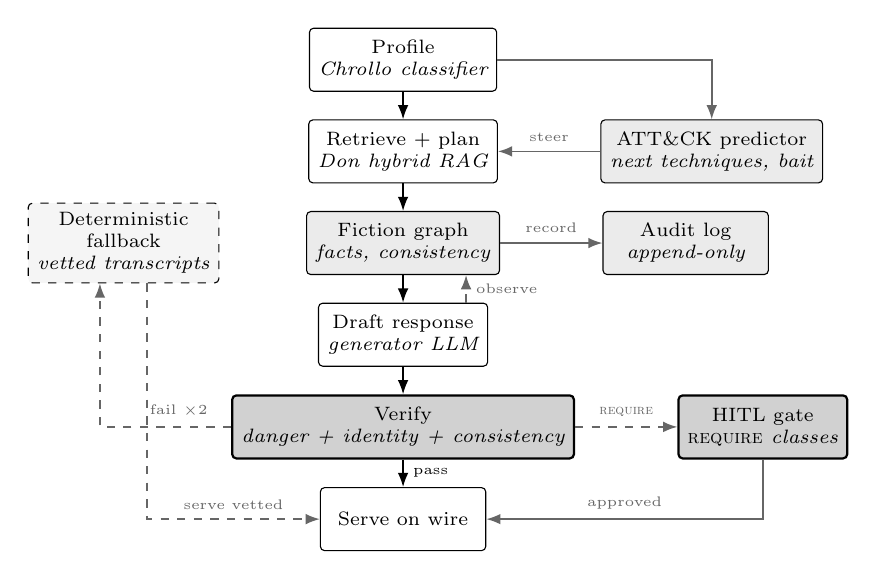
\begin{tikzpicture}[
  node distance=3.5mm and 5mm,
  stage/.style={draw, rounded corners=1.5pt, minimum height=8mm, minimum width=21mm, align=center, font=\scriptsize},
  store/.style={stage, fill=black!8},
  gate/.style={stage, fill=black!18, thick},
  fail/.style={draw, dashed, rounded corners=1.5pt, minimum height=8mm, align=center, font=\scriptsize, fill=black!4},
  arr/.style={-{Latex[length=1.8mm]}, semithick},
  farr/.style={arr, dashed, black!60}
]
% Main serving path (top to bottom)
\node[stage] (profile) {Profile\\ \scriptsize\itshape Chrollo classifier};
\node[stage, below=of profile] (retrieve) {Retrieve + plan\\ \scriptsize\itshape Don hybrid RAG};
\node[store, below=of retrieve] (graph) {Fiction graph\\ \scriptsize\itshape facts, consistency};
\node[stage, below=of graph] (draft) {Draft response\\ \scriptsize\itshape generator LLM};
\node[gate, below=of draft] (verify) {Verify\\ \scriptsize\itshape danger + identity + consistency};
\node[stage, below=of verify] (serve) {Serve on wire};

% Side stores
\node[store, right=13mm of retrieve] (mitre) {\attck predictor\\ \scriptsize\itshape next techniques, bait};
\node[store, right=13mm of graph] (audit) {Audit log\\ \scriptsize\itshape append-only};
\node[gate, right=13mm of verify] (hitl) {HITL gate\\ \scriptsize\itshape \textsc{require} classes};

% Failure path
\node[fail, left=11mm of graph] (fallback) {Deterministic\\ fallback\\ \scriptsize\itshape vetted transcripts};

% Main path arrows (vertical spine)
\draw[arr] (profile) -- (retrieve);
\draw[arr] (retrieve) -- (graph);
\draw[arr] (graph) -- (draft);
\draw[arr] (draft) -- (verify);
\draw[arr] (verify) -- (serve) node[midway, right, font=\tiny] {pass};

% Failure arrows: orthogonal, left corridor, offset anchors
\draw[farr] (verify.west) -| ([xshift=-3mm]fallback.south)
  node[pos=0.2, above, font=\tiny] {fail $\times$2};
\draw[farr] ([xshift=3mm]fallback.south) |- (serve.west)
  node[pos=0.75, above, font=\tiny] {serve vetted};

% Approval arrow: right corridor into serve.east
\draw[arr, black!60] (hitl.south) |- (serve.east)
  node[pos=0.75, above, font=\tiny] {approved};
\draw[farr] (verify.east) -- (hitl.west) node[midway, above, font=\tiny] {\textsc{require}};

% Feedback / context arrows: right gap, offset entry into graph.south
\draw[arr, black!60] (mitre) -- (retrieve) node[midway, above, font=\tiny] {steer};
\draw[arr, black!60] (profile.east) -| (mitre.north);
\draw[arr, black!60] (graph.east) -- (audit.west) node[midway, above, font=\tiny] {record};
\draw[farr] ([xshift=8mm]draft.north) -- ([xshift=8mm]graph.south)
  node[midway, right, font=\tiny] {observe};
\end{tikzpicture}

\caption{The verified deception loop. A session enters through the
behavioral classifier (Chrollo), which routes it to a per-class deception
policy. The retrieval engine (Don) grounds the policy in CTI; the fiction
graph binds every host fact; the generator drafts under the binding; the
verifier checks the draft against the graph before serving. Dashed paths
are failure paths: verification failure falls back to deterministic
transcripts, and content flagged \textsc{require} pauses at the
human-in-the-loop gate.}
\label{fig:architecture}
\end{figure*}

\subsection{The Fiction Graph}
\label{sec:graph}
Every fact the honeypot projects about itself (hostname, kernel, listening
ports, installed databases, user accounts) is stored as a
subject--predicate--value triple in a per-session \emph{fiction graph}.
The graph is seeded from the host identity at session start and grows by
two mechanisms: \emph{declaration}, when the deception plan asserts a new
fact, and \emph{observation}, when a served response is scanned and any
host-like entities it emitted are extracted and recorded. Observation is
the mechanism that binds the LLM to the recorded state: whatever the generator said the
host is, the graph now remembers, and the next draft must agree with it.

A triple carries its source, and consistency is checked at the predicate
level: two declarations of the same predicate with different values raise
a contradiction, with normalization tuned to distinguish a genuine
conflict from a benign surface variant (a hostname is not contradicted by
its fully qualified form). When a contradiction is detected, the graph
records it and the verification node treats any draft resting on the
contradicted fact as unservable. The fiction graph is what turns G2 from
an aspiration into a data structure; the serving-time invariant below
states the consistency condition it enforces and its attacker-visible
scope.

\subsection{Verified Generation}
\label{sec:verify}
Generation is a draft, not a decision. The generator (a provider-hosted
LLM) receives the session context, the deception plan, a compact
serialization of the fiction graph (a \emph{fact block}), and the
steering context: the \attck techniques predicted to follow the
attacker's observed sequence, together with bait artifacts matched to
those techniques. The prediction uses the \attck tactic ordering to
propose the attacker's likely next moves (G1's steering half).

Before a draft reaches the wire it passes five checks:
\begin{enumerate}
\item \textbf{Danger scan.} A pattern gate rejects credential-material,
offensive-content, and real-secret signatures; one considered exemption: a
bare token a real command would print (the correct answer to
\texttt{whoami} is one word) is not chatter.
\item \textbf{Identity pin.} Identity-revealing commands answer from the
persona's pinned identity---a novice never answers \texttt{whoami} with
\texttt{root}, the hostname never changes mid-session, a root-prompting
attempt is rejected. The C1 battery carries a dedicated proof.
\item \textbf{Consistency check.} Host-like entities are observed into the
fiction graph; a contradictory draft is rejected with the contradiction
recorded.
\item \textbf{Supported-claim check.} On the declared deterministic
command surface, the draft must \emph{contain} the correct
answer---hedging, echoing, or omitting is a rejection; outside the
declared surface the check is silent, so open-ended recall is untouched.
\item \textbf{Terminal sanity.} Shell-shaped responses that answer a
command with sentence-like prose instead of executable output are
rejected.
\end{enumerate}
A draft that fails any check is retried once with the violation fed back;
a second failure triggers fallback. The checks were selected by one
criterion: each must be a \emph{decision procedure} over the draft,
decidable, cheap, and deterministic, because a verifier that itself calls
a model would only relocate the trust problem it exists to solve. What
verification deliberately does not certify is quality. A draft can pass
all five checks and still be unpersuasive; plausibility is not
decidable, and the paper does not pretend otherwise. The division of
labor is the point: the loop's machinery enforces the three properties
of the three safety constraints machine-checkably, and the consensus study of
\S\ref{sec:rq3} assesses the deception quality that only evaluation can
measure. This is the mechanism behind the zero-unverified-serves claim
evaluated in \S\ref{sec:evaluation}. The serving sequence above gives
the full loop; its fallback arm carries G4 and its \textsc{Require}
branch carries G3.

\subsection{Cross-Session Host Fiction}
\label{sec:hostfiction}
The per-session fiction buys bounded blast radius
at a measured price: a returning attacker is shown a fresh world, and
none of the session verifier's checks can see drift \emph{between}
sessions. The host-fiction layer closes exactly that gap without
widening the blast radius. It is host-keyed rather than session-keyed:
at an attacker's first contact with a host, its identity is pinned and
provisioned into every consumer --- the persona prompt is rebuilt from
the pinned identity (removing a class of contradictory-instruction
failures where prompt and verifier disagreed), the session graph is
seeded authoritatively for verification, and the fallback template
inherits the same identity. Facts observed in a session are promoted to
the host store only when they passed verification (fail-closed: an
unverified session never binds a host fact), and every subsequent
session against the same host is cross-checked against the promoted
set by a session-verifier wrapper that rejects on cross-session
contradiction. Reconnect policies are configurable: a returning
connection can share the pinned graph outright, or start a promoted
session whose facts are cross-checked against the host.

The layer is measured, not merely present. On identical deterministic
drift scenarios (reconnect drift, beyond-identity drift, cross-skill
host swap, simultaneous contradiction, repetition controls), the
session-scoped verifier alone catches 1 of 4 cross-session drift drafts;
both host-fiction policies catch 4 of 4 with 0 of 7 benign re-query
false rejections (\path{cross_session_consistency_bench.json}). The
three misses of the session-scoped baseline are invisible to it by
construction --- facts asserted in a previous session simply are not in
current-session state --- and per-skill identities name different hosts,
so a reclassified returning attacker would otherwise be shown a
different machine. On benign traffic the layer is free: paired over the
full 218-query workload, store-on versus store-off serves byte-identical
strings on every row (paired per-row delta exactly $0.0000$;
\path{external_baseline_hostfiction_comparison.json}), so cross-session
consistency is added at zero quality cost on the evaluated surface.

\subsection{Human-in-the-Loop Gate}
\label{sec:hitl}
Content classes whose compromise value is high (deployed credentials,
for instance) are marked \textsc{require} in the deception policy. When a
response would serve such content, the loop pauses and the decision is
surfaced to the operator through an audit interface that records the
context, the draft, and the decision. Every gate decision is persisted to
an append-only audit log, which \S\ref{sec:evaluation} uses as a
correctness and governance record.
The gate encodes a governance position: the system may \emph{draft}
deception, but a human decides when the deception includes trap
material (G3). The gate exists for the operator's stake, not the
attacker's: canary bait is safe to serve by construction, but it is
still an active measure whose use an operator may be required to
authorize; the audit record of that authorization leaves the system
defensible after the fact. The require-level branch is also where the
credential-deployment decisions in the benchmark trail
(Appendix~\ref{app:audit}) were made.

\subsection{Deterministic Fallback}
\label{sec:fallback}
Every scenario class has a vetted deterministic transcript: hand-written,
fiction-consistent bait and response templates (credential hunts, service
enumerations, exfiltration decoys) whose secrets are registered canaries.
When generation fails, the provider times out, verification rejects twice,
or the model refuses the persona, the loop serves the deterministic
transcript for the scenario instead. The fallback is not an admission of
defeat; it is the safety floor that makes the LLM path safe to enable.
The A5 ablation checks that the system is \emph{equivalent} through the
fallback path, and the design of the canary registration is what allows
the consensus study to distinguish deployed bait from accidental leaks.

Session state beyond identity facts replays the same discipline. A
filesystem ledger records the bytes served for every read command and
replays them verbatim when the same path is read again; time-varying
ambient content (process identifiers, timestamps, clock outputs) is not
stored but generated by hashing a per-session seed through a template,
so re-reads are identical within a session while sessions differ
plausibly from one another, and a mutating command invalidates the
affected entries so subsequent reads reflect the mutation. This ledger,
not the generative path, is what the byte-identical replay component of
the C1 result (\S\ref{sec:rq2}) exercises: determinism on re-query is a
property of how session state is stored and replayed, and the design
keeps it decoupled from generation.
The fallback also carries a hidden load: it defines the system's floor
under failure. Because the fallback serves the same fiction the generator
would have, an attacker cannot distinguish a degraded session from a
healthy one by content alone; the availability
property of G4 thereby becomes a deception property, not merely a reliability one.
What the fallback gives up is the generator's adaptivity: a fallback
session answers within its scenario's script and steers no further,
which is the correct trade only because the loop treats it as a floor
beneath the LLM path rather than the path itself.

\section{Formal Properties and Adversarial Analysis}
\label{sec:formal}

The mechanism walk of \S\ref{sec:design} described what the loop does;
this section states what the loop \emph{enforces} and prices what an
adaptive adversary can still do to it. The two are paired deliberately:
each invariant names the evaluation that stresses it, and each attack
channel closes against one of the invariants.

\subsection{The Serving-Time Consistency Invariant}
\label{sec:invariant}

The fiction graph (\S\ref{sec:design}) turns G2 from an aspiration into a
data structure. We state the consistency condition it enforces, together
with its induction and its measured stress test.

\begin{property}[Serving-time fiction consistency]
\label{prop:consistency}
Let $\mathcal{G}$ be a session's fiction graph and $F(\mathcal{G})$ the set
of host facts derivable from it, two facts conflicting when they assign
conflicting normalized values to one predicate. Write $\sigma_t$ for the
served response at turn $t$ and $E(\sigma_t)$ for the host facts the
verifier extracts from the draft --- all expressible in the graph's
declared fact schema (host identity, kernel, services, credential
shapes). The loop maintains the invariant
\begin{equation*}
E(\sigma_t) \not\pitchfork F(\mathcal{G}_{t-1}) \ \wedge \ F(\mathcal{G}_t) = \mathrm{cl}\big(F(\mathcal{G}_{t-1}) \cup E(\sigma_t)\big)
\end{equation*}
for every served turn: no served response conflicts with the facts the
session has already committed to, and the graph absorbs each served
response's facts before the next draft. Verification failure breaks the
left conjunct \emph{before} serving, so the violated draft is never
observable to the attacker; the failure path serves deterministic vetted
content instead. The argument is a short induction. The empty graph is
trivially conflict-free. If the invariant holds at turn $t-1$, then any
draft whose emitted facts conflict with $\mathrm{cl}(F(\mathcal{G}_{t-1}))$ is rejected
before serving, and only conflict-free drafts are observed into the
closure; the closure of a conflict-free set remains conflict-free, so the
invariant holds at $t$. The failure path preserves the invariant by
construction: fallback transcripts emit only vetted facts, pre-registered
against the seed graph. Because $\mathrm{cl}$ is the transitive closure of the
graph's predicate conflicts, the invariant extends from
single turns to sessions: an attacker who re-queries any fact under any
phrasing receives a value consistent with every prior turn. The C1
benchmark (\S\ref{sec:rq2}) tests exactly this: zero contradictions over
45 adversarial re-queries, with the upper confidence bound $0.079$.
The guarantee is deliberately relative to that schema: a contradiction
phrased so that $E$ extracts nothing within it is not visible to this
property. This is the same scoping discipline as the supported-claim
surface below --- certification where the check is decidable, an
explicit boundary where it is not, rather than a universal claim over
arbitrary semantic content.
\end{property}

Property~\ref{prop:consistency} is a soundness statement over the
declared fact schema: no schema-recognized conflicting fact is served.
It deliberately says nothing about \emph{completeness} --- a
draft that answers nothing also asserts nothing false. The verification
surface therefore extends with a complementary, explicitly scoped
requirement. For a declared set of commands whose real-Linux output is
deterministic given the machine identity (identity queries, kernel and
OS facts, echo, uptime shape, date shape, the OS-release file), the
served response \emph{must contain} the identity-correct answer:
hedging, echoing the query back, or omitting the answer is a finding,
not a pass, and the draft is rejected by the same gate. The surface is
\emph{closed per claim type} --- each command has a deterministic
extractor and an exact or shape-level match rule, and no claim outside
the declared set incurs the requirement --- so the extension cannot
collapse recall on the open-ended remainder of attacker behavior, which
the consistency property continues to guard. Internally, the extension
fails closed: an error inside a claim checker yields a finding, never a
silent pass. The extension is measured as well as declared: a
123-case labeled red-team suite for the verifier
(\path{verifier_redteam_supported_claims.json}) reports precision and
recall of $1.0$ on the supported-claim stratum under the deployed
fail-closed configuration --- nine violations (wrong identity, query
echo, hedging, wrong OS release) rejected, and nine correct-answer and
outside-surface probes passed with no false rejections. The combined
statement is: on the declared supported-claim surface, every serve is
correct; elsewhere, every schema-recognized factual claim is
consistency-checked.

\subsection{The Verified-Serve Algorithm}
\label{sec:algorithm}

\begin{algorithm}[t]
\caption{Verified-serve loop (per attacker turn $x$)}
\label{alg:loop}
\begin{algorithmic}[1]
\Require session state $\sigma$, fiction graph $\mathcal{G}_\sigma$, attacker turn $x$, policy $\pi$
\State $c \gets \textsc{Classify}(x, \sigma)$ \Comment{behavioral class (Chrollo)}
\State $\pi \gets \textsc{Plan}(c, \textsc{Retrieve}(x, \sigma))$ \Comment{grounded plan (Don)}
\State $B \gets \textsc{FactBlock}(\mathcal{G}_\sigma)$ \Comment{graph serialization}
\For{$\mathit{try} \in \{1, 2\}$}
  \State $d \gets \textsc{Draft}(x, \pi, B, \textsc{Steer}(\pi))$ \Comment{provider LLM}
  \State $\mathcal{G}' \gets \textsc{Observe}(\mathcal{G}_\sigma, d)$ \Comment{absorb emitted host facts}
  \If{$\textsc{DangerScan}(d) \ \vee$}
     \State \hspace{\algorithmicindent} $\textsc{IdentityPin}(d, \pi) = \bot \ \vee$
     \State \hspace{\algorithmicindent} $\textsc{Consistent}(\mathcal{G}', d) = \bot \ \vee$
     \State \hspace{\algorithmicindent} $\textsc{SupportedClaim}(d, \pi) = \bot \ \vee$
     \State \hspace{\algorithmicindent} $\textsc{TerminalSanity}(d) = \bot$ \Comment{§\ref{sec:verify}}
     \State \hspace{\algorithmicindent} \textbf{continue} \Comment{retry with violation fed back}
  \EndIf
  \If{$\textsc{Require}(d, \pi)$} \Comment{high-stakes content class}
     \State \textbf{return} \textsc{HITLGate}$(d, \pi)$ \Comment{G3: human decides}
  \EndIf
  \State \textbf{return} $d$ \Comment{verified: serve}
\EndFor
\State \textbf{return} \textsc{Fallback}$(\pi)$ \Comment{G4: vetted deterministic transcript}
\end{algorithmic}
\end{algorithm}

Algorithm~\ref{alg:loop} gathers the serving path into one place: the
five decision-procedure checks of \S\ref{sec:verify} form the reject
arm, the \textsc{Require} branch carries G3, and the fallback arm
carries G4. Every branch is deterministic given the draft; the only
nondeterminism in the loop is the provider model itself, which is
exactly the component the checks exist to bound.

\subsection{Attacking the Loop}
\label{sec:attack}
An adaptive adversary (\S\ref{sec:threatmodel}) who has read this
section has two footholds, and the design prices both. The first is the
\emph{observation channel}: a served response's facts enter the graph,
so an attacker who induces the honeypot to commit a lie has poisoned one
session's world. The design contains this rather than prevents it.
Commitment is one-way on purpose: the graph absorbs what was served,
never what was merely drafted, so a rejected draft leaves no trace, and
the session lifetime bounds the poisoned world to the attacker who
created it. What the channel cannot do is leak true state, because the
graph contains no true state to leak; every triple originates in the
deception plan, the seed identity, or a prior verified serve.

The second foothold is the \emph{steering channel}. Predicted next
techniques and matched bait reach the generator as context, and
attacker-controlled input influences what is retrieved and predicted;
an attacker who knows this could shape their own session to steer bait
of their choosing. Three facts bound the exposure. Bait is drawn from a
closed canary-registered catalog, so the worst case is an attacker
obtaining a credential that was designed to be obtained and is designed
to be traced. Retrieval runs over a curated corpus, not open text, so
corpus poisoning requires access the threat model denies
(\S\ref{sec:threatmodel}). And the HITL gate sits between every
high-stakes deployment and the wire, so steering the machinery still
requires persuading a human. The residual risk is stated plainly: a
sufficiently informed attacker can make the honeypot commit deeper to
one fiction branch than the operator intended, at no safety cost and at
the cost only of that session's plan flexibility.

\section{Implementation}
\label{sec:implementation}

We describe the implementation at the level of detail needed to reproduce
the evaluation; the complete system is open-source.\footnote{Repository
link omitted for review.}

\subsection{Session Profiler}
The behavioral classifier is a random forest (scikit-learn) over ten
features grouped in two families: behavioral (regex hit counts for
persistence, privilege escalation, credential access, lateral movement,
scanning, and custom tooling) and structural (command complexity,
tool-usage diversity, unique-command ratio, and inter-command timing
variance). It predicts one of four attacker classes (novice, intermediate,
expert, APT-grade) with a confidence score; low-confidence sessions route
to the conservative policy. Feature normalization is $z$-score scaling
with $k$-NN imputation ($k{=}5$) for missing values.

\subsection{Retrieval Engine}
Don fuses a FAISS dense index with BM25 lexical retrieval over the curated
CTI corpus, weighting dense and sparse scores $\alpha{=}0.7$ and
$\beta{=}0.3$, and maps retrieved activity to \attck techniques through a
dedicated threat mapper with evidence citations attached to every
analysis. Documents are screened before indexing to blunt corpus
poisoning~\cite{chaudhari2024,jia2025}: per-document provenance checks,
indicator sanity validation, and quarantine of documents that fail
screening. Generative calls run through a provider gateway with output
length caps and low temperature, and the retrieval prompt constrains the
model to cite retrieved documents.

\subsection{Deception Engine and Persona Management}
The deception engine (\emph{Hisoka}) binds the plan to the persona: a
persona manager selects the projected host identity from the attacker
class; a response generator produces the drafts that \S\ref{sec:verify}
verifies; an artifact injector plants honeytoken
material whose secrets are registered canaries (so any later
appearance of a canary in outbound traffic is attributable to a bait
interaction by construction, not a leak); and an engagement tracker measures dwell time per session. Skill tier maps to
prompt strategy: novice-facing surfaces are low-friction and
exploitation-shaped; expert-facing surfaces introduce subtle
inconsistencies that force verification loops, exposing toolchain
signals~\cite{kouremetis2024}. Session state lives in Redis with
TTL-based expiry.

\subsection{Cross-Session Memory}
Session-scoped state expires by design; attacker memory persists by
design. A separate memory layer (mem0ai) maintains per-attacker
profiles keyed by source-IP hash: each turn is distilled into a typed
natural-language trace, extracted facts accumulate in the profile, and
the profile is re-injected into retrieval and generation on subsequent
sessions, with a configurable idle aging window (30 days in our
deployment). The separation matters because long-horizon behavior
(slow credential testing, repeat scanner visits, multi-day
lateral-movement staging) is exactly the signal that static emulation
cannot exploit. Profiles are created on first observation and exercised
by integration tests against a mocked backend.

\subsection{Deployment and Cost}
The full stack (honeypot listeners, retrieval, orchestration, monitoring)
runs on a single commodity host: 2~vCPU, ${\sim}4$~GB RAM, Docker
containers for the honeypot services. The deployment used for the
evaluation is reachable only over a tailnet, a scope restriction
discussed in \S\ref{sec:discussion}. Generative components
call provider-hosted models through an API gateway; no local GPU is
required, and the entire serving path adds no infrastructure beyond the
single host. A model-churn watcher probes the provider catalog and quota
twice daily, logging drift (a wired model disappearing) as a hard failure;
the churn this watcher caught during the evaluation period is part of the
provider-fragility discussion in \S\ref{sec:discussion}.

\subsection{Software Stack}
\begin{itemize}
\item \textbf{Honeypot listeners:} Cowrie-compatible SSH, plus HTTP and
Telnet services behind the same session interface.
\item \textbf{Retrieval:} FAISS + BM25 hybrid.
\item \textbf{Orchestration:} Python 3.12 async pipeline; the verified
loop is an explicit state machine with per-node state persistence.
\item \textbf{Session state:} Redis (TTL-scoped); attacker memory: mem0ai.
\item \textbf{Monitoring:} Prometheus metrics per component; append-only
HITL audit log.
\end{itemize}

\section{Evaluation}
\label{sec:evaluation}

% Results figures, rendered from the persisted artifacts:
% bootstrap_ci.json (suite means and 95% CIs), stability_run1_vs_run2.json (run pairs).
% Values resolve through figures/generated_values.tex, which scripts/gen_sp_figures.py
% writes from those artifacts; run `python scripts/gen_sp_figures.py --check` to prove
% this figure still agrees with them.
% Layout discipline: the top panel shows point estimates + intervals only
% (no filled bars under the whiskers), the bottom panel's legend lives
% below the axis (never over the bars), and both panels share the same
% value range so the stacked scales read as one.
% GENERATED by scripts/gen_sp_figures.py -- do not edit by hand.
% Every plotted number in the S&P figures resolves through this file, so a
% figure cannot silently disagree with the artifact it claims to show.
% Regenerate:  python scripts/gen_sp_figures.py
% Verify:      python scripts/gen_sp_figures.py --check
% Sources:
%   results/bootstrap_ci.json
%   results/stability_run1_vs_run2.json
%   results/b4_baseline_zodiac_20260922.json
%   results/model_quality/chrollo_calibration.json
%   results/sp2027_rescue/behavior_trajectory_benchmark.json

\def\RaginLiveTechnique{0.9598}
\def\RaginLiveTechniqueErrLo{0.0122}
\def\RaginLiveTechniqueErrHi{0.0122}
\def\RaginLiveActor{0.8500}
\def\RaginLiveActorErrLo{0.0000}
\def\RaginLiveActorErrHi{0.0000}
\def\RaginLivePersona{0.7325}
\def\RaginLivePersonaErrLo{0.0587}
\def\RaginLivePersonaErrHi{0.0558}
\def\RaginLiveComposite{0.8796}
\def\RaginLiveCompositeErrLo{0.0224}
\def\RaginLiveCompositeErrHi{0.0204}
\def\RaginLivePersonaRunTwo{0.7504}
\def\RaginLiveCompositeRunTwo{0.8845}
\def\RaginPersonaRunDelta{0.018}
\def\RaginTechDelta{0.317}
\def\RaginTechDeltaLo{0.162}
\def\RaginTechDeltaHi{0.480}
\def\RaginActorDelta{0.140}
\def\RaginActorDeltaLo{0.083}
\def\RaginActorDeltaHi{0.197}
\def\RaginPersonaNullDelta{0.005}
\def\RaginPersonaNullDeltaLo{-0.047}
\def\RaginPersonaNullDeltaHi{0.057}
\def\RaginOverallDelta{0.154}
\def\RaginOverallDeltaLo{0.092}
\def\RaginOverallDeltaHi{0.221}
\def\RaginGroundingTtpCount{35}
\def\RaginNoGroundingTtpCount{0}
\def\RaginRoutingBefore{0.8875}
\def\RaginRoutingAfter{0.955}

\begin{figure}[t]
\centering
\begin{tikzpicture}
\begin{axis}[
  name=ax1,
  width=0.96\linewidth,
  height=4.9cm,
  xmin=0.55, xmax=1.02,
  y axis line style={draw=none},
  axis x line*=bottom,
  axis y line*=left,
  ytick=data,
  yticklabels={Composite,Persona,CTI actor$^{\dagger}$,CTI technique},
  y dir=reverse,
  xlabel={score (95\% CI)},
  xlabel style={font=\footnotesize},
  tick label style={font=\footnotesize},
  enlarge y limits=0.6,
  grid=major,
  grid style={black!10},
  clip=false
]
% point estimates and bootstrap 95% CIs from bootstrap_ci.json;
% only marks + intervals: no bars beneath the whiskers
\addplot+[only marks, mark=|, mark size=3.4, mark options={thick,black},
  error bars/.cd, x dir=both, x explicit] coordinates {
  (\RaginLiveTechnique,3) +- (\RaginLiveTechniqueErrLo,\RaginLiveTechniqueErrHi)
  (\RaginLiveActor,2) +- (\RaginLiveActorErrLo,\RaginLiveActorErrHi)
  (\RaginLivePersona,1) +- (\RaginLivePersonaErrLo,\RaginLivePersonaErrHi)
  (\RaginLiveComposite,0) +- (\RaginLiveCompositeErrLo,\RaginLiveCompositeErrHi)
};
% run-2 overlay: open markers (point estimates from stability_run1_vs_run2.json;
% per-suite CIs were not computed for run 2, so none are drawn)
\addplot+[only marks, mark=o, mark size=1.9, mark options={semithick,black!60}] coordinates {
  (\RaginLiveTechnique,3)
  (\RaginLiveActor,2)
  (\RaginLivePersonaRunTwo,1)
  (\RaginLiveCompositeRunTwo,0)
};
\end{axis}
\end{tikzpicture}

\vspace{2mm}

\begin{tikzpicture}
\begin{axis}[
  name=ax2,
  width=0.96\linewidth,
  height=4.9cm,
  ybar=1.5pt,
  bar width=9pt,
  ymin=0.55, ymax=1.0,
  symbolic x coords={CTI technique,CTI actor,Persona,Composite},
  xtick=data,
  ylabel={mean score},
  ylabel style={font=\footnotesize},
  tick label style={font=\footnotesize},
  ymajorgrids,
  grid style={black!10},
  enlarge x limits=0.25,
  legend style={font=\scriptsize, at={(0.5,-0.16)}, anchor=north, legend columns=2, draw=none, fill=none},
  legend cell align={left},
]
% run 1 vs run 2 from stability_run1_vs_run2.json
\addplot+[black!35, fill=black!35] coordinates {
  (CTI technique,\RaginLiveTechnique) (CTI actor,\RaginLiveActor) (Persona,\RaginLivePersona) (Composite,\RaginLiveComposite)
};
\addplot+[black!70, fill=black!70, pattern=north east lines] coordinates {
  (CTI technique,\RaginLiveTechnique) (CTI actor,\RaginLiveActor) (Persona,\RaginLivePersonaRunTwo) (Composite,\RaginLiveCompositeRunTwo)
};
\legend{run 1, run 2}
\end{axis}
\end{tikzpicture}
\caption{Live-campaign results from the persisted artifacts (identical
deterministic-strata bars across runs are the finding, not a plotting
error). All four plotted values are the \emph{both-channel} operational
score of Table~\ref{tab:live}, which fuses the served-text and CTI-analysis
channels; they are not served-quality results, and the echo-guarded bounds
for the same rows are 0.479 technique and 0.243 actor.
\emph{Top:}
suite means with bootstrap 95\% confidence intervals; open markers mark
the independent second run's point estimates, and the actor interval is
degenerate ($^{\dagger}$) because the actor rubric assigns the same
score to every row, so uncertainty is carried by the Wilson pass-rate
interval instead (Table~\ref{tab:live}). \emph{Bottom:} two independent
218-query campaigns; the deterministic CTI strata replicate exactly and
only the LLM-judged persona stratum moves, by $+\RaginPersonaRunDelta$.}
\label{fig:results}
\end{figure}


The evaluation asks whether each mechanism the design introduces
contributes measurably. We organize it by the four research questions of
\S\ref{sec:intro}: the value of grounding (RQ1), consistency and safety
under adversarial interaction (RQ2), deception quality under
multi-persona model evaluation (RQ3), and the escalation pricing of each
intelligence rung
(RQ4), followed by run-to-run stability and threats to
validity. Every quantitative claim in this section is traceable to a
persisted artifact in the released benchmark suite; where an interval is
reported it is a bootstrap 95\% confidence interval computed over paired
rows or over case clusters, as noted at the point of use.

\subsection{Experimental Setup}
\label{sec:setup}

\subsubsection{Testbed}
The evaluation testbed is the production single-host deployment
(2~vCPU, ${\sim}4$~GB RAM), driven by an evaluation harness that runs on a
separate workstation (12~vCPU, 15\,GiB RAM; \S\ref{app:repro}); the two
share no state. Generative
components use two model families from one free-tier provider: a generator
for deception drafts and a judge model for evaluation, chosen from a
different family than the generator. The provider catalog and quota are
probed by a scheduled watcher; its history shows the catalog drifting
under observation --- wired models disappearing from the listing during
and after the study, and unwired models appearing in or vanishing from
it between consecutive twice-daily probes --- alongside availability
events, a quota-exhaustion window and transient gateway outages; every
event logged by the watcher and absorbed by the fallback path of
\S\ref{sec:fallback}.

\subsubsection{Workloads}
Three query suites exercise the loop end to end:
\emph{CTI-technique} (123 queries asking how specific \attck techniques
are abused, scored on grounded technique coverage),
\emph{CTI-actor} (35 queries on named threat-actor behavior, scored on
attribution quality), and \emph{persona-realism} (60 interactive sessions
driven by scripted attacker personas, scored by an LLM judge on
host-believability rubrics). Each suite runs through the full verified
loop with HITL auditing enabled. The scenario sets are fixed and released,
so every run below is a re-run of the same 218 sessions.

\subsubsection{Metrics}
Suite scores are normalized to $[0,1]$ with a per-scenario pass threshold;
composite is the row-weighted mean. For the ablation we report
paired-difference bootstrap CIs, pairing rows by scenario across arms. For
consistency we report contradiction rate over targeted re-queries. For
deception quality we report a 1--5 rubric consensus over three evaluator
personas, scored on five dimensions: \emph{deception realism} (would the
output pass as the claimed service), \emph{persona consistency} (does
content match the attacker's skill tier), \emph{TTP accuracy} (are the
extracted \attck mappings correct and complete), \emph{engagement} (does
the response invite continued interaction rather than dead-ending), and
\emph{artifact safety} (is served credential material registered canary
bait rather than leakage). Each evaluator also records a rationale per
dimension; these rationales are what located the harness defect and the
fiction contradiction reported below. Every score in this section
additionally declares its \emph{scoring channel}: the \textbf{served-text}
channel grades what the attacker receives; the \textbf{analysis} channel
grades what the pipeline's retrieval layer identified, which is never
served. The two are never combined silently; where a composite max()es
both (the technique and actor strata of the reference campaign), we say
so at the point of use, and \S\ref{sec:scorer-audit} reports each channel
separately under a corrected, echo-guarded served-text rubric.

\subsection{RQ1: Does Grounding Change What the Honeypot Detects?}
\label{sec:rq1}

We run the full 30-scenario-per-suite workload twice through the live
loop: once with retrieval grounding enabled and once with Don bypassed
(prompts otherwise identical), pairing every scenario across arms. This
is a direct test of G1 under the paired design that answers the
circularity concern: the same corpus, the same prompts, only retrieval
removed.

\begin{table}[t]
\centering
\caption{Paired RAG-vs-no-RAG differential (180 observations = 90
matched pairs, one per scenario per arm; 95\% bootstrap CIs computed
over the 90 per-pair differences). Persona realism is predicted to be
retrieval-independent, and is.}
\label{tab:b4}
\begin{tabular}{lccc}
\toprule
Suite & RAG & No-RAG & $\Delta$ (95\% CI) \\
\midrule
CTI technique & 0.950 & 0.633 & $+0.317$ $[+0.162, +0.480]$ \\
CTI actor     & 0.850 & 0.710 & $+0.140$ $[+0.083, +0.197]$ \\
Persona       & 0.833 & 0.828 & $+0.005$ $[-0.047, +0.057]$ \\
\midrule
Overall (90 pairs) & & & $+0.154$ $[+0.092, +0.221]$ \\
\bottomrule
\end{tabular}
\end{table}
% Paired grounding effect (RAG minus No-RAG) per suite with 95% bootstrap
% CIs, from b4_baseline_zodiac_20260922.json (the same numbers as
% Table~tab:b4). Filled markers: intervals excluding zero. Open marker:
% the persona stratum, whose interval straddles zero exactly as the
% architecture predicts. Compiled statically; no results directory needed.
% GENERATED by scripts/gen_sp_figures.py -- do not edit by hand.
% Every plotted number in the S&P figures resolves through this file, so a
% figure cannot silently disagree with the artifact it claims to show.
% Regenerate:  python scripts/gen_sp_figures.py
% Verify:      python scripts/gen_sp_figures.py --check
% Sources:
%   results/bootstrap_ci.json
%   results/stability_run1_vs_run2.json
%   results/b4_baseline_zodiac_20260922.json
%   results/model_quality/chrollo_calibration.json
%   results/sp2027_rescue/behavior_trajectory_benchmark.json

\def\RaginLiveTechnique{0.9598}
\def\RaginLiveTechniqueErrLo{0.0122}
\def\RaginLiveTechniqueErrHi{0.0122}
\def\RaginLiveActor{0.8500}
\def\RaginLiveActorErrLo{0.0000}
\def\RaginLiveActorErrHi{0.0000}
\def\RaginLivePersona{0.7325}
\def\RaginLivePersonaErrLo{0.0587}
\def\RaginLivePersonaErrHi{0.0558}
\def\RaginLiveComposite{0.8796}
\def\RaginLiveCompositeErrLo{0.0224}
\def\RaginLiveCompositeErrHi{0.0204}
\def\RaginLivePersonaRunTwo{0.7504}
\def\RaginLiveCompositeRunTwo{0.8845}
\def\RaginPersonaRunDelta{0.018}
\def\RaginTechDelta{0.317}
\def\RaginTechDeltaLo{0.162}
\def\RaginTechDeltaHi{0.480}
\def\RaginActorDelta{0.140}
\def\RaginActorDeltaLo{0.083}
\def\RaginActorDeltaHi{0.197}
\def\RaginPersonaNullDelta{0.005}
\def\RaginPersonaNullDeltaLo{-0.047}
\def\RaginPersonaNullDeltaHi{0.057}
\def\RaginOverallDelta{0.154}
\def\RaginOverallDeltaLo{0.092}
\def\RaginOverallDeltaHi{0.221}
\def\RaginGroundingTtpCount{35}
\def\RaginNoGroundingTtpCount{0}
\def\RaginRoutingBefore{0.8875}
\def\RaginRoutingAfter{0.955}

\begin{figure}[t]
\centering
\begin{tikzpicture}[
  font=\scriptsize,
  dot/.style={circle, fill=black, inner sep=1.5pt},
  nul/.style={circle, draw=black, fill=white, inner sep=1.5pt, thick},
  arr/.style={-{Latex[length=1.6mm]}, semithick, black!55}
]
  % zero reference
  \draw[black!45] (0,0.5) -- (0,-3.2);
  \node[font=\tiny, text=black!60, anchor=east] at (-0.05,0.5) {$\Delta=0$};

  % CTI technique: +0.317 [+0.162, +0.480]
  \node[anchor=east] at (-0.25,0) {CTI technique};
  \draw[black!70] (1.62,0) -- (4.80,0);
  \draw[black!70] (1.62,-0.13) -- (1.62,0.13);
  \draw[black!70] (4.80,-0.13) -- (4.80,0.13);
  \node[dot] at (3.17,0) {};

  % CTI actor: +0.140 [+0.083, +0.197]
  \node[anchor=east] at (-0.25,-0.95) {CTI actor};
  \draw[black!70] (0.83,-0.95) -- (1.97,-0.95);
  \draw[black!70] (0.83,-1.08) -- (0.83,-0.82);
  \draw[black!70] (1.97,-1.08) -- (1.97,-0.82);
  \node[dot] at (1.40,-0.95) {};

  % Persona (predicted null): +0.005 [-0.047, +0.057]
  \node[anchor=east] at (-0.25,-1.9) {Persona};
  \draw[black!70] (-0.47,-1.9) -- (0.57,-1.9);
  \draw[black!70] (-0.47,-2.03) -- (-0.47,-1.77);
  \draw[black!70] (0.57,-2.03) -- (0.57,-1.77);
  \node[nul] at (0.05,-1.9) {};

  % Overall
  \draw[black!25, dashed] (-0.25,-2.5) -- (5.0,-2.5);
  \node[anchor=east] at (-0.25,-3.0) {Overall (90 pairs)};
  \draw[black!70] (0.92,-3.0) -- (2.21,-3.0);
  \draw[black!70] (0.92,-3.13) -- (0.92,-2.87);
  \draw[black!70] (2.21,-3.13) -- (2.21,-2.87);
  \node[dot] at (1.54,-3.0) {};

  % axis
  \draw[arr] (0,-3.65) -- (5.1,-3.65);
  \foreach \x/\l in {0/0, 1/{+0.1}, 2/{+0.2}, 3/{+0.3}, 4/{+0.4}} {
    \draw[black!55] (\x,-3.58) -- (\x,-3.72)
        node[below, font=\tiny, text=black!60] {\l};
  }
\end{tikzpicture}
\caption{Paired grounding differential (RAG $-$ No-RAG) per suite with
95\% bootstrap CIs over 90 scenario pairs (numbers in
Table~\ref{tab:b4}). Filled markers: intervals excluding zero -- $+\RaginTechDelta$
on technique detection and $+\RaginActorDelta$ on actor attribution. The open
marker is the persona stratum, whose interval straddles zero exactly as
the architecture predicts: host believability is produced by the
deception engine and the fiction graph, not by threat-intelligence
retrieval. The mechanism behind the technique effect is starker than
the mean: the grounded arm yields \RaginGroundingTtpCount{} TTP detections spanning 21 distinct
techniques, while the ungrounded arm yields none.}
\label{fig:grounding}
\end{figure}


Table~\ref{tab:b4} and Figure~\ref{fig:grounding} show the result.
Grounding lifts technique detection
by $+0.317$ and actor attribution by $+0.140$, both intervals excluding
zero. The mechanism claim is starker: the grounded arm detects 35 TTPs
(21 distinct techniques) across the campaign; the ungrounded arm detects
none. The persona
stratum is the informative null: its interval straddles zero, exactly as
the architecture predicts, because host-believability is produced by the
deception engine and the fiction graph, not by threat-intelligence
retrieval. An ablation that produced only wins would look manufactured;
this one discriminates. The mechanism claim is consistent at the
deployment level: the grounded arm passes 30 of 30 technique scenarios;
the ungrounded arm passes 22 of 30, failing precisely the
synthesis-shaped scenarios (multi-step technique chains, actor-conditioned
campaign context) where static templates have nothing to say.

\emph{Effect under the guarded scorer.} The campaign's technique and
actor composites combine the served-text and analysis channels; under the
echo-guarded served-text-only rubric of \S\ref{sec:scorer-audit}, the
fallback-dominated rows that the raw rubric credited score zero, and the
absolute served-text levels of both arms drop. The grounding contrast
itself is not restated numerically there because the ablation artifact
predates full-transcript persistence and cannot be re-derived offline;
what is preserved is the mechanism asymmetry the guarded measurement
makes visible: TTP detection (35 detections vs.\ 0) is an analysis-channel
capability and is unchanged by the guard, while the persona-realism null
--- the stratum the architecture predicts should not move with retrieval
--- is untouched by it. A healthy-generation-window re-run with full
transcript persistence, restating the served-text differential explicitly
under the current (guarded) scorer, is released as the protocol's next
step; one arm has already been re-run natively under that scorer --- the
scripted cowrie baseline at composite $0.0006$, unchanged, as it
produces no echoes (\path{external_baseline_cowrie_guarded_rerun.json}).

\emph{Takeaway: grounding is responsible for the intelligence the system
produces, and the ablation localizes the effect to exactly the suites
that need it.}

\subsection{RQ2: Consistency and Safety Under Adversarial Interaction}
\label{sec:rq2}

\subsubsection{Fiction-graph consistency}
We re-query 45 facts across live sessions (kernel versions, hostnames,
listening services, database engines, credentials) using adversarial
phrasings designed to induce drift, then compare each response against
the session's fiction graph. The graph-full configuration serves zero
contradictions across 45 re-queries (95\% CI upper bound $0.079$, i.e.,
the true contradiction rate is below 8\% even at the interval's
pessimistic edge), replays byte-identically, records
zero pinned-identity violations, and serves no response after a failed
verification verdict. The no-enforcement baseline provides none of these
properties (verifier coverage 45/45 turns versus 0). One disclosure
bounds the claim: the C1 artifact records verifier verdicts per turn
but not serve-path labels, and 11.9\% of campaign serves are
deterministic-path (Table~\ref{tab:live}), so some re-query turns may
be template serves for which consistency is a property of the vetted
library rather than graph-enforced generation --- and the byte-identical
determinism across adversarial phrasings (rate $1.0$) is itself
consistent with a deterministic component in this stratum. A
serve-path-stamped re-run remains future work; the zero-contradiction
result itself is unaffected, since both serve paths are verified or
vetted by construction. One failure this
benchmark caught during development is instructive: a benign
\texttt{uname} re-query was briefly flagged as a contradiction because
the extraction layer matched a distribution alias against the pinned
kernel string, a false contradiction we fixed and regression-locked; the
verifier now fails safe (unverifiable facts are rewritten or withheld,
never served on faith). Cross-session drift --- assertions that
contradict facts the same attacker was shown in a \emph{previous}
session --- is invisible to the session-scoped verifier by construction
(1 of 4 drift drafts caught); the host-fiction layer of
\S\ref{sec:hostfiction} closes it (4 of 4 caught, 0 of 7 benign false
rejections) at exactly zero paired cost over the 218-row workload.

\subsubsection{Predictive steering}
The \attck predictor converts observed techniques into ranked next-move
candidates, and the deception plan attaches bait for the top candidates.
Across 10 predictions grounded in the session corpora, top-3 next-technique
accuracy is $0.9$, top-1 is $0.5$, MRR is $0.667$, and the
steered bait reaches the plan in $0.9$ of sessions. The A2 ablation
confirms the bait signal comes from the steering context: removing it
collapses steer-context-to-plan from $0.9$ to $0.0$, and bait-matched
reach --- the fraction of plans whose bait covers the predicted next
technique --- from $0.4$ to $0.0$.

\subsubsection{Mechanism ablations}
\begin{table}[t]
\centering
\caption{Ablation battery over the eight ground-truth scenarios
(persisted audit counts). Each removed mechanism should cost the system
the property it was added to provide; A5 tests path equivalence, not
degradation.}
\label{tab:ablations}
\small
\setlength{\tabcolsep}{4pt}
\begin{tabular}{>{\raggedright\arraybackslash}p{2.4cm}>{\raggedright\arraybackslash}p{3.3cm}>{\raggedright\arraybackslash}p{1.9cm}}
\toprule
Configuration & Observable in audit & Cost \\
\midrule
full (reference) & 8/8 verified serves; strategy and & -- \\
 & fiction blocks in 8/8 plans; 3 gated & \\
A1 no fiction graph & fiction block in 0/8 plans & plan loses \\
 & & fact binding \\
A2 no bait steering & strategy block in 0/8 plans; & steer and bait \\
 & & reach $0.9/0.4 \to 0$ \\
A3 no verifier & 8/8 served with no verdict & zero verified \\
 & & serves \\
A4 no HITL gate & 3 require-class contents served & governance \\
 & ungated & lost \\
A5 no graph engine & 8/8 verified, same serves & none (equivalent) \\
\bottomrule
\end{tabular}
\end{table}
Table~\ref{tab:ablations} summarizes the battery. Each row removes one
mechanism and tests the corresponding design goal from
\S\ref{sec:design} that motivated it;
all four degrade as designed, and the linear fallback
path is behaviorally equivalent when the graph adds no information (G4).

\subsubsection{Induced verifier failures}
The clean campaign is a serving-safety workload, not a sensitivity test:
its zero failed-verification serves cannot establish that the verifier would
reject a bad draft. We therefore ran an independent authored-draft matrix
through the same post-fix verifier. The canonical deterministic red-team
suite contains 105 cases (78 reject and 27 pass cases) and achieves
$P=R=1.000$ on every check. The live matrix varies the author family and
keeps the verifier fixed; it is a stress test of extraction and vocabulary,
not an end-to-end attacker campaign.

\begin{table}[t]
\centering
\caption{Post-fix verifier stress test across authored draft families. The
live rows are valid drafts, not served sessions; the llama row includes 48
explicitly disclosed substitute-author fills. Recall intervals are 95\%
case-cluster bootstrap intervals (10{,}000 resamples of cases, seed
\texttt{20261008}); drafts within a case are not independent, so the
draft-level intervals they replace are not used.}
\label{tab:verifier-cross-family}
\scriptsize
\setlength{\tabcolsep}{3pt}
\begin{tabular}{lrrrrr}
\toprule
Author family & Cases & Drafts & Precision & Recall & 95\% recall CI \\
\midrule
space-bunny-free & 89 & 261 & 1.000 & 0.959 & [0.926, 0.985] \\
deepseek-v4-flash-free & 80 & 236 & 1.000 & 0.983 & [0.961, 1.000] \\
llama-3.3-70b & 94 & 281 & 0.916 & 0.898 & [0.848, 0.943] \\
\midrule
Deterministic canonical suite & 105 & -- & 1.000 & 1.000 & -- \\
\bottomrule
\end{tabular}
\end{table}

The residual misses concentrate in author-side consistency drift and
author-specific tell vocabulary; the llama row also contains disclosed
substitute-author outputs, so it is a robustness bound rather than a clean
model ranking. This distinction matters operationally: the 218-row campaign
establishes that the deployed loop did not serve after a failed verdict,
whereas Table~\ref{tab:verifier-cross-family} establishes that induced bad
drafts can be rejected with bounded, model-dependent recall. Together they
support a fail-closed serving contract without claiming universal semantic
coverage.

\subsubsection{Live campaign}
\begin{table}[t]
\centering
\caption{Live 218-query campaign (verified loop, per-row bootstrap CIs).
Scores are the declared both-channel composite (\S\ref{sec:scorer-audit}):
served text max()'d with the CTI-analysis channel. Zero errors;
218/218 sessions engaged; 218/218 correct persona assignments; 132 TTPs
(67 unique) detected with zero false-positive CTI alerts (counted
against the scripted workload's expected techniques). Serve-path
provenance: latency-derived split 88.1\% verified-generation serves,
11.9\% vetted deterministic (the loop's designed deterministic rung),
zero fail-safe fallback serves; the content-level scorer audit bounds
the template-anchored CTI share higher (\S\ref{sec:scorer-audit}). Echo-zeroed lower bounds on the same rows: technique
$0.479$, actor $0.243$; guarded served-text means on the row-matched
audited surface: $0.057$/$0.000$ (\S\ref{sec:scorer-audit}).}
\label{tab:live}
\begin{tabular}{lccc}
\toprule
Suite & $n$ & Mean & 95\% CI \\
\midrule
CTI technique & 123 & 0.960 & $[0.948, 0.972]$ \\
CTI actor     & 35  & 0.850 & $[0.850, 0.850]^\dagger$ \\
Persona       & 60  & 0.733 & $[0.674, 0.788]$ \\
\midrule
Composite     & 218 & 0.880 & $[0.857, 0.900]$ \\
\bottomrule
\multicolumn{4}{l}{\footnotesize $^\dagger$Degenerate by construction: the actor rubric assigns the} \\
\multicolumn{4}{l}{\footnotesize same composite to every row, so the mean's bootstrap} \\
\multicolumn{4}{l}{\footnotesize interval carries no width; pass-rate uncertainty is} \\
\multicolumn{4}{l}{\footnotesize reported instead (Wilson $[0.901, 1.0]$; the technique} \\
\multicolumn{4}{l}{\footnotesize stratum is also $123/123$, Wilson $[0.970, 1.0]$).} \\
\end{tabular}
\end{table}
Table~\ref{tab:live} reports the full campaign and
Figure~\ref{fig:results} (top) renders the suite means with their
intervals. The persona stratum is
the binding floor: 58 of 60 sessions pass, and the failures are
timeout-shaped turns under provider safety-alignment pressure rather
than deception failures, consistent with the provider-fragility
limits stated in \S\ref{sec:conclusion}.

\emph{Serve-path provenance.} Zero errors should not be read as the
deterministic path absorbing the campaign. In the released system, the
graph nodes stamp each served row with an explicit path label at the
node that produced the served bytes (verified generation, retry,
deterministic fast-path, or fail-safe fallback); the latency split
(\path{serve_provenance.json}) attributes 88.1\% of run 1's serves
(87.2\% of run 2's) to the verified-generation path and the remainder to
vetted deterministic content, shifting only at 10\,s thresholds
(sensitivity is persisted), and survives as a cross-check on the
stamped labels rather than the primary instrument. One correction
applies to \emph{earlier} serve-path tallies, including this split:
the deceiver's gateway-outage, unsafe-retry, and template-anchored
responses previously carried no marker and were counted as
verified-generation; they are now labeled deterministic template
serves (\texttt{TEMPLATE\_FALLBACK\_VERIFIED}), and pre-correction
tallies in retained artifacts are re-interpreted accordingly rather
than rewritten. The scorer-validity audit of \S\ref{sec:scorer-audit}
is what surfaced this hole, and it is quantitative: on the audited
CTI surface, roughly one hundred rows served echo-shaped template text
while carrying verified-generation labels --- so the latency-derived
split must be read as a lower bound on the deterministic share, not as
the audited content-level count. Decisively,
\emph{Fallback serves are zero}: no row in either run records a failed
verifier verdict, so the fail-safe template swap never engaged -- the
vetted share is the loop's designed deterministic rung doing its job on
protocol-shaped turns, not degradation. Subject to the marker
correction above, the composite of Table~\ref{tab:live} is a declared
both-channel measure: a latency-derived minority of serves are vetted
deterministic content, a larger template-anchored share on the CTI
surface is bounded by the corrected served-text strata of
\S\ref{sec:scorer-audit}, and the remainder is verified generative
quality.

\emph{Auditing the persona judge.} Because the persona stratum's
automated judge is a deterministic realism rubric, it can be audited
exhaustively offline against the transcripts it scored -- a check the
LLM-as-a-judge literature recommends for learned judges
\cite{zheng2024}. Two systematic errors surfaced
(\path{live_benchmark_judge_panel_corrected.json}). First, \emph{bait
blindness}: on a credential-hunt query, the loop served registered
canary credentials -- the correct deception outcome under the
canary-registry construction of \S\ref{sec:design}, which bars real
secrets from the serving path -- and the rubric, which rewards realism
signals and penalizes brevity, scored the concise bait deployment
$0.25$. Second, \emph{harness contamination}: one row whose transcript
is a session-harness echo bug (the query re-emitted as a shell command,
then ``command not found'') entered the deception mean at $0.0$ despite
measuring nothing about deception. The audit re-scores both runs with
three corrections: reclassifying harness artifacts out of the deception
mean, applying the credential-bait floor ($0.85$) to rows that deploy
key-shaped canaries on credential-hunt queries, and rounding persisted
floats. The correction is small in aggregate -- persona means move
$0.733\to0.756$ and $0.750\to0.762$ -- but it is directional and it
removes a bias against the system's best behavior: the canary-bias
magnitude, the score mass the judge had moved against correct bait
deployments, is 1.35 points across the two runs. The rubric was patched
consistently (deployment floor applied after penalties), the audit
script and corrected judge carry regression tests, and both raw and
corrected means are released rather than silently substituted.

\emph{Takeaway: the consistency and safety properties hold under targeted
adversarial pressure; A1--A4 each remove exactly the property the
mechanism was introduced to enforce, while A5 validates safe path
equivalence when the graph contributes no additional information.}

\subsection{RQ3: Deception Quality Under Multi-Persona Model Evaluation}
\label{sec:rq3}

An LLM honeypot can be internally consistent and still be unconvincing,
so we score the end product. Eight ground-truth scenarios (credential
hunts, service enumeration, cloud-metadata probes, exfiltration staging)
are executed live and the full transcripts are scored on a 1--5 rubric
(deception realism, persona consistency, TTP accuracy, artifact safety)
by three evaluator personas. Consensus is the per-scenario mean across
evaluators; exact agreement across the three personas is $0.750$ -- a
within-model consistency figure, since all three personas share one
judge model (Appendix~\ref{app:rubrics}), not inter-annotator agreement
in the human-study sense. The consensus score is
$\mathbf{3.86/5}$, with all eight scenarios at or above the $3.0$ acceptance bar (the
rubric's midpoint, fixed before per-scenario inspection), five of eight
at 4 or above, and the best scenario (service enumeration) at $4.20$.
Table~\ref{tab:consensus} gives the per-scenario consensus with the
rubric profile.

\begin{table}[t]
\centering
\caption{Per-scenario consensus (mean of three evaluator personas over
the 1--5 rubric). The rubric profile of the weakest scenario locates the
weakness in persona realism and artifact safety, not in the deception's
technique accuracy.}
\label{tab:consensus}
\small
\setlength{\tabcolsep}{3.5pt}
\resizebox{\columnwidth}{!}{%
\begin{tabular}{lcccccc}
\toprule
Scenario & Decep. & Pers. & TTP & Eng. & Art. & Overall \\
\midrule
GT-001 whoami        & 4.0 & 4.0 & 5.0 & 4.0 & 3.7 & 4.1 \\
GT-002 show creds    & 4.0 & 4.0 & 5.0 & 4.0 & 4.0 & 4.2 \\
GT-003 privesc       & 4.0 & 3.7 & 5.0 & 4.0 & 3.3 & 4.0 \\
GT-004 IMDS/SSRF     & 4.0 & 4.0 & 4.3 & 4.0 & 3.3 & 3.9 \\
GT-005 SQLi          & 2.3 & 2.7 & 5.0 & 4.0 & 1.0 & 3.0 \\
GT-006 services      & 4.0 & 4.0 & 5.0 & 4.0 & 4.0 & 4.2 \\
GT-007 reverse shell & 3.0 & 3.0 & 3.0 & 4.0 & 4.0 & 3.4 \\
GT-008 shadow dump   & 4.0 & 4.0 & 4.7 & 4.3 & 3.7 & 4.1 \\
\midrule
\textbf{Consensus} & & & & & & \textbf{3.86} \\
\bottomrule
\end{tabular}%
}
\end{table}

Three protocol details matter for interpreting the number. First,
evaluators score complete transcripts, not excerpts; an earlier scoring
pass on truncated transcripts was rerun after we fixed the harness. Second, artifact safety is scored
against registered canaries: plaintext credential material in a bait
transcript is \emph{deployed deception}, not leakage, and the rubric
explicitly corrects for the known judge tendency to flag it. Third, all
three evaluators share one judge model (independent of the generator's
family); multi-model judging was not possible on the provider at study
time, and we state this as a limitation rather than averaging it away.
Fourth, a blinded real-vs-honeypot \emph{discrimination} study --- human
raters labeling mixed packets of genuine de-identified real-Linux
sessions against the systems compared here --- is preregistered, with
its protocol and packets released alongside the artifact; we claim
nothing from it here and treat its completion as the human-grounded
test of the deception claim.

The weakest scenario ($3.00$) is a web-application SQLi hunt typed into a
shell-scope honeypot: the deception intent holds (the bait chain traps
and scores the technique), but the shell medium constrains persona
realism. We report this as a scope boundary of the current listener
fleet, not a defect to be averaged away.

\emph{Takeaway: the deception holds a three-evaluator consensus above
the $3.0$ bar on every scenario, with the failure modes named rather
than smoothed.}

\subsection{RQ4: Pricing the Ladder -- Adaptive Kind-Awareness and Its
Fold-Down}
\label{sec:jeveval}

The top rung of the ladder (\S\ref{sec:ladder}) is adaptive: a
kind-aware assessment layer (\emph{Jev}) that reads session behavior and
returns the attack kind and skill tier that the routing and deception
layers should act on. We price it in three experiments, each with its
artifact released.

\emph{Assessment quality on real logs.} On 13 replayed sessions drawn
from real Cowrie logs, the baseline pipeline without kind-awareness
correctly assessed 0; with it, 12 of 13
(\path{jev_real_logs_eval.json}). The one miss was a session whose
recorded behavior was consistent with two kinds; we report the miss
rather than resolve it by hindsight.

\emph{Steering effect.} A 200-session stratified A/B on routing decisions
(50 per skill tier, \path{jev_ab_eval.json}) shows the ladder's descent
in action. In the first pipeline revision, kind-aware enrichment lifted
routing accuracy from 69.5\% (139/200) to 91.5\% (183/200), fixing all 44
assessed APT misroutes (a free-tier rate limit capped the assessment
layer at 44/200 sessions) with zero regressions. The final revision then reproduced that
entire gain deterministically: an apt skill-map repair, a weighted
behavior-severity floor, and an n-gram-feature retrain of the classifier
(0.8875 $\to$ 0.9550) reach 100\% with the assessment layer contributing
zero marginal accuracy ($\Delta = 0.0$, $n=200$; no assessment output
was available on any of the 200 sessions, \texttt{jev\_available}$=0$ in
the released artifact). Both arms sit at the
pass ceiling, so this comparison alone cannot separate ``the floor
already covers everything the assessment layer adds'' from ``the
benchmark contains nothing left to cover'': a routing decision is scored
correct when it meets the tier's risk floor, and the floor mechanism
meets it on every sampled session. We therefore census the full
400-session held-out corpus for the stratum where the comparison is
informative -- sessions whose deterministic routing lands below the tier
floor (\path{jev_hard_subset.json}). The stratum is small: six sessions,
all APT-tier, all exactly one rung under floor, drawn from the
classifier's lower-confidence tail (mean confidence 0.53 versus 0.75
corpus-wide). On this stratum the assessment layer was evaluated live:
one session was assessed and rescued (baseline \emph{high} $\to$
assessment \emph{critical} $\to$ final at floor); the remaining five
returned empty assessments after provider refusals -- the free-tier
endpoint refuses security-shaped payloads, a behavior a controlled
probe confirmed (benign command states serve; attacker-tooling states
receive HTTP 403). A structured retry measurement (four attempts per
row, spaced) recovered none of the five, and the refusal pattern
varied across executions -- the rescue itself appears to have been a
transient pass rather than a stable availability mode. The top rung's marginal
effect on routing is therefore unmeasured in both directions, for two
compounding reasons: informative sessions are rare under the current
floor, and they are exactly the sessions the provider is least willing
to assess. The removal stands on its measured record -- zero marginal
effect on every row the benchmark resolves, zero regression risk added
by removal, and a provider dependency eliminated -- but the bound is
stated rather than claimed away: the result is \emph{no measurable
marginal effect at this benchmark's resolution}, not general subsumption.
Figure~\ref{fig:funnel} traces the census; Table~\ref{tab:hardsunset}
summarizes it alongside the live arm.
% The fold-down evidence funnel: the full held-out corpus narrowed to the
% stratum where the routing comparison is informative, then the live arm's
% outcomes. Census values from the released jev_hard_subset.json; the
% 0/5 retry outcome is the structured retry measurement described in the
% text. Compiled statically so the figure needs no results directory.
\begin{figure}[t]
\centering
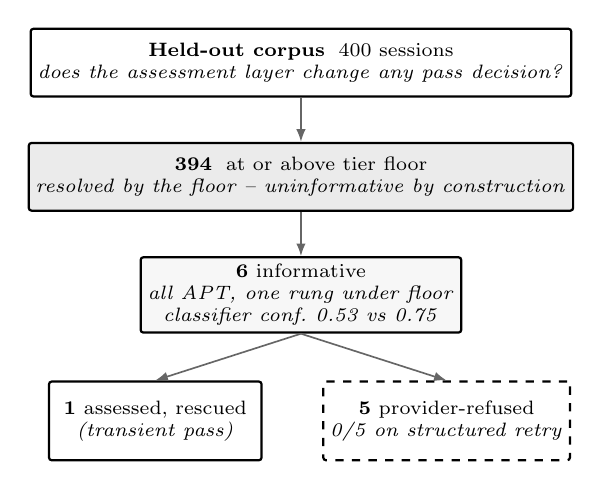
\begin{tikzpicture}[
  font=\scriptsize,
  stage/.style={draw, rounded corners=1pt, thick, align=center,
                inner sep=2.5pt, minimum height=8.6mm},
  dead/.style={stage, fill=black!8},
  live/.style={stage, fill=black!3},
  resc/.style={stage, minimum height=10mm},
  refu/.style={stage, minimum height=10mm, dashed},
  arr/.style={-{Latex[length=1.6mm]}, semithick, black!60}
]
  % 1. full corpus
  \node[stage, minimum width=62mm] (corpus) at (0,0)
       {\textbf{Held-out corpus}\; 400 sessions\\
        \textit{does the assessment layer change any pass decision?}};
  % 2. resolved branch (the inert majority)
  \node[dead, minimum width=50mm] (floor) at (0,-1.45)
       {\textbf{394}\; at or above tier floor\\
        \textit{resolved by the floor -- uninformative by construction}};
  % 3. the informative stratum
  \node[live, minimum width=36mm] (info) at (0,-2.95)
       {\textbf{6} informative\\
        \textit{all APT, one rung under floor}\\
        \textit{classifier conf.\ 0.53 vs 0.75}};
  % 4. live-arm outcomes
  \node[resc, minimum width=27mm] (r1) at (-1.85,-4.55)
       {\textbf{1} assessed, rescued\\ \textit{(transient pass)}};
  \node[refu, minimum width=27mm] (r5) at (1.85,-4.55)
       {\textbf{5} provider-refused\\ \textit{0/5 on structured retry}};
  \draw[arr] (corpus) -- (floor);
  \draw[arr] (floor) -- (info);
  \draw[arr] (info.south) -- (r1.north);
  \draw[arr] (info.south) -- (r5.north);
\end{tikzpicture}
\caption{The fold-down evidence funnel (census in
Table~\ref{tab:hardsunset}). Deterministic routing resolves 394 of 400
held-out sessions at the tier floor before the assessment layer is
consulted; the six sessions below floor form the only stratum where the
top rung can change a pass decision, and the live arm's evidence there
is one transient rescue and five provider refusals that did not recover
on a structured retry.}
\label{fig:funnel}
\end{figure}


\emph{A second rung presents fold-down pressure.} The ladder audit's
pricing protocol has now been run against a second intelligent rung: the
retrieval-engine choice. A 50-query retrieval benchmark with 5 runs per
query (\path{stat_eval/summary.json}), Wilcoxon-signed-rank over paired
query means with Holm correction, compares the LLM-fusion retrieval
engine against deterministic BM25 (sparse): the two are statistically
indistinguishable on precision@5 ($p_{\text{Holm}}{=}0.51$),
recall@20 ($0.32$), and MRR ($0.085$), and the deterministic engine is
\emph{significantly better} on NDCG@10 ($p_{\text{Holm}}{=}0.022$, mean
difference $-0.161$ against the LLM engine). This is fold-down pressure
at benchmark resolution on the retrieval rung --- distinct from the
RQ1 grounding contrast, which compares retrieval against \emph{none} and
is large; here the comparison is between retrieval engines, and the
intelligent one buys nothing the cheap one does not already provide on
three of four metrics. Unlike the routing rung, this fold-down is
\emph{priced but not executed}: acting on it requires a paired
pipeline-level A/B (graph engine vs.\ BM25 through the full verified
loop on the 218-query workload), which we release as the protocol's next
step rather than claiming the removal now. The design rule therefore has
two priced instances and one executed removal.
The availability result strengthens the removal on its own terms: a
rung that returns empty precisely on APT-shaped sessions is a liability
on the highest-stakes traffic, independent of what its accuracy would
be when it answers.

\begin{table}[t]
\centering
\caption{Fold-down hard-subset census (the released
\texttt{jev\_hard\_subset.json}). The informative stratum for the routing
comparison is the set of held-out sessions whose deterministic routing
lands below the tier's risk floor; on every other row the assessment
layer cannot change the pass decision by construction. The live arm
assessed one of six informative sessions; the other five were refused
by the provider and did not recover on a structured retry protocol
(see text).}
\label{tab:hardsunset}
\small
\setlength{\tabcolsep}{4pt}
\begin{tabular}{@{}lc@{}}
\toprule
Census over the full held-out corpus & \\
(400 sessions) & \\
\midrule
Floor at or above tier floor & 394 \\
Informative (baseline below floor) & 6 \\
\quad tier & all APT \\
\quad under-floor depth & 1 rung \\
\quad classifier conf.\ (inf.\ / corpus) & 0.53 / 0.75 \\
\midrule
Live assessment arm (6 sessions) & \\
\midrule
Assessed and rescued (transient) & 1 \\
Unavailable; 0/5 recovered on structured retry & 5 \\
\bottomrule
\end{tabular}
\end{table}

\emph{Deception effect in closed loop.} Paired closed-loop replays pit a
simulated LLM attacker against the deception engine with and without
kind-aware guidance (\path{jev_dwell_replay_llm_REPORT.md}; 97.8\%
LLM-backed gateway calls, verified by a canary echo probe after an
earlier run was found to have silently template-fallen back). Bait
markers surfaced to the attacker rose from 4 to 9 (+125\%) across the
five error-free family pairs drawn from seven attempted families (two
excluded for attacker-LLM provider errors; $n{=}5$; no power claim). Dwell time
did not move: 34 vs.\ 33 turns
in the clean paired comparison. The report's own mechanism analysis
explains the null: in both arms, nearly every early leave cites
inconsistent fictional filesystem state -- a cautious attacker reads
inconsistency as a trap signal, so response consistency, not deception
style, is the binding constraint. This is precisely why the fiction
graph and verifier sit below the adaptive layer in the ladder: the
consistency rungs are load-bearing for every rung above them.

\emph{Takeaway: the top rung buys assessment coverage and bait exposure,
not dwell time -- and its routing contribution, unresolvable at the
benchmark's ceiling and unavailable on the rows that matter most, was
compiled down to a deterministic floor. The clearest signal in this
evaluation about where intelligence belongs is also the one stated with
its resolution bound.}

\subsection{Scorer-Validity Audit and Two-Channel Metrics}
\label{sec:scorer-audit}

Automated scorers are components of the measurement pipeline, and this
paper's own provenance rules apply to them: a scorer that has never been
checked against an independent standard is a claim, not an instrument. We
therefore audited the served-text rubric directly. A stratified sample of
the 218-query workload was re-served through the identical pipeline and
double-annotated under blinding: two independent annotator models with
fixed identities scored each row's served text against a taxonomy pinned
to \attck{} Enterprise v19.1 (vendored STIX, hash-locked), with no access
to gold labels or pipeline scores; a third annotator adjudicated every
disagreement (none unresolved). Annotator agreement is substantial on
technique identification (Cohen's $\kappa=0.866$); the actor stratum's
low raw agreement decomposes into confidence-threshold skew, not topic
disagreement. The audit's substantive finding is about the scorer:
string-matching the served text credits a technique identifier or actor
name appearing \emph{anywhere} in a response, and deterministic fallback
responses echo the attacker's query verbatim --- so on fallback-heavy
runs the rubric scored error text as grounded content. All
scorer-on-topic/annotator-off-topic conflicts (67 technique, 33 actor rows)
were exactly this echo class.

The correction is mechanical and persisted: when the served text echoes
the query verbatim and carries a fallback marker, the score is zero,
matching the annotators' labels. Echo-guarded rescores move the
served-text means on the audited surface from $0.524$ to $0.057$
(technique) and $0.680$ to $0.000$ (actor) --- the honest measurement of
a fallback-dominated serve surface --- while scorer-vs-annotator agreement
jumps from $\kappa=-0.187$ to $+0.349$ (technique) and $0.048$ to
$0.914$ (actor). The deception-realism stratum is unchanged ($0.649$):
its rubric already penalized echoes. Table~\ref{tab:cti-audit} reports
the audit; Table~\ref{tab:two-channel} reports the corrected two-channel
measurement; Table~\ref{tab:baseline-served-text} places the external
baselines on the same declared channel.

% Auto-generated by scripts/gen_two_channel_tables.py — 2026-09-28
% Declared scoring channels (never mix without labeling):
%   served_text  = deception realism (what the attacker receives)
%   cti_analysis = intelligence value (Don extraction; NOT served)
% Served-text numbers are echo-guarded (blinded-audit correction,
%   results/cti_manual_audit.json); the audited surface was proven
%   row-matched to the two-channel reference run (218/218 pre-guard score equality).

\subsection{Two-Channel Evaluation}

Every metric below declares its \emph{scoring channel}. The \textbf{served-text} channel scores what the attacker actually receives; the \textbf{CTI-analysis} channel scores what the pipeline identified (Don extraction), which is never shown to the attacker. The two answer different questions---deception realism vs.\ intelligence value---and are never combined into a single composite.

The served-text rubric originally credited a technique identifier or actor name appearing anywhere in the response. A double-annotated blinded audit (\S\ref{sec:scorer-audit}) found that on fallback-heavy runs the served surface is dominated by deterministic templates that echo the query verbatim, so the raw rubric credited error text (97 of 218 rows corrected). Both raw and guarded columns are shown: the gap itself is a finding about the serve surface.

\begin{table}[t]
\centering
\caption{Two-channel metrics of the verified RAGIN pipeline (generator: gateway default (glm-5.3-flash-free)). Served text is shown raw (the echo-crediting rubric) and echo-guarded (post-audit); the guarded column is canonical. The deception surface deliberately answers CTI-style questions with machine transcripts, not technique essays; the intelligence value lives in the analysis channel. Guarded numbers are computed on the audited surface, proven row-matched to this run by pre-guard score equality on all 218 rows (\texttt{cti\_manual\_audit.json}).}
\label{tab:two-channel}
\resizebox{\columnwidth}{!}{%
\begin{tabular}{lccc}
\toprule
Suite & Served (raw) & Served (guarded) & CTI analysis \\
\midrule
Technique identification (123 q) & 0.524 & 0.057 & 0.960 \\
Actor attribution (35 q) & 0.680 & 0.000 & 0.850 \\
Persona realism (60 q) & 0.649 & 0.649 & -- \\
\bottomrule
\end{tabular}%
}
\end{table}

\begin{table}[t]
\centering
\caption{External baselines on the 218-query workload (generator: deepseek-v4-flash-free for all LLM arms). \textbf{All scores are served-text channel under the raw (pre-guard) rubric}---the deception quality an attacker experiences. Paired per-row deltas are scorer-invariant: the verified loop serves byte-identical strings to the no-verifier arm on all 218 rows (paired delta 0.000), and the host-fiction layer adds cross-session consistency at exactly zero quality cost (paired per-row delta 0.000). Absolute levels on fallback-heavy runs shift under the echo guard (Table~\ref{tab:two-channel}); the grounding and consistency contrasts do not.}
\label{tab:baseline-served-text}
\begin{tabular}{lc}
\toprule
Arm & Served-text composite \\
\midrule
Vanilla Cowrie (no LLM) & 0.001 \\
Stateful LLM (HoneyGPT/LLM-SSHH) & 0.070 \\
Bare LLM (unverified) & 0.502 \\
RAGIN w/o verifier & 0.618 \\
RAGIN full (verified loop) & 0.618 \\
RAGIN full + host fiction & 0.618 \\
\bottomrule
\end{tabular}
\end{table}

\begin{table}[t]
\centering
\caption{Blinded annotator audit of the automated scorers (\S\ref{sec:scorer-audit}): two independent blinded annotators (fixed-identity free-tier models, no gold labels, no pipeline scores), third-annotator adjudication, taxonomy pinned to \\attck{} Enterprise v19.1 (vendored STIX, sha256-locked). Scorer-vs-annotator agreement is Cohen's $\kappa$ between the automated channel verdicts and the adjudicated annotator labels, before/after the echo guard. All disagreements were adjudicated; none unresolved.}
\label{tab:cti-audit}
\small
\setlength{\tabcolsep}{3.5pt}
\resizebox{\columnwidth}{!}{%
\begin{tabular}{@{}lccccc@{}}
\toprule
Suite & $n$ & $\kappa$ (A,B) & strict F1 (A/B) & adjud.\ A/B/neither & scorer-vs-annot.\ $\kappa$ pre$\to$post \\
\midrule
Technique identification & 123 & 0.866 ($n$=123) & 0.732/0.732 & 4/3/0 & -0.187$\to$0.349 \\
Actor attribution & 35 & 0.160 ($n$=35) & 0.771/0.765 & 2/4/0 & 0.048$\to$0.914 \\
Persona realism & 60 & 0.072 ($n$=60) & --/-- & 4/8/4 & 0.099$\to$0.099 \\
\bottomrule
\end{tabular}%
}
\end{table}

% Echo-guard correction provenance: results/cti_manual_audit.json (echo_guard_correction): 97 rows changed; served avg pre->post: technique 0.5236->0.0569, actor 0.68->0.0, deception 0.6492->0.6492 (persona scorer already penalized echoes). Post-guard scorer-vs-annotator kappa: technique -0.187->+0.349, actor 0.048->0.914 (scorer now agrees with the annotator models). Ladder paired per-row deltas are scorer-invariant (byte-identical served strings across compared arms on the decisive rows).

% Historical note (Sep-22 campaign): its official technique (0.960) and actor (0.850) averages were BOTH-channel (served text max analysis). Its served-text-only equivalents are 0.493 / 0.666 under the raw rubric. Do not compare across channels; see results/technique_rubric_diff_investigation.json.


The model-coherent ladder is the stronger comparison: all LLM arms use
\texttt{deepseek-v4-flash-free}. A bare LLM scores $0.502$ on the raw
served-text composite, while grounded RAGIN without verification scores
$0.618$ ($+0.116$). The full verifier holds the same $0.618$ quality while
changing all 218 rows from \texttt{GENERATED\_UNVERIFIED} to verified or
vetted paths; the host-fiction layer also remains at $0.618$ but catches
cross-session drift in 4/4 cases versus 1/4 for session-only state. This is
the current result behind the security claim: verification contributes a
serving boundary at quality parity, while grounding contributes the measured
quality increase. The older 0.960/0.850 technique/actor headline is retained
only as a both-channel historical campaign result and is not used to compare
the model-coherent arms.

Three properties survive the correction unscaled. First, the verified
loop's zero-unverified-serve property is structural, not scored: the
served surface is produced by verified drafts or vetted fallbacks
regardless of how a rubric grades the text. Second, the ladder's paired
per-row deltas are scorer-invariant where the compared arms serve
byte-identical strings (verified vs.\ no-verifier, host-fiction on vs.\ off); absolute levels shift under the guard, the contrasts do not.
Third, the analysis channel --- what Don extracted, never shown to an
attacker --- reproduces the campaign's intelligence yield ($0.960$
technique, $0.850$ actor) independently of the serve surface. The two
channels answer different questions, and \S\ref{sec:rq1}'s grounding
contrast is restated on both: TTP detection is an analysis-channel
capability; the served deception surface deliberately answers CTI-style
questions with machine transcripts rather than technique essays.

One limitation of the correction must be stated rather than waved
away: the external-baseline checkpoints of
Table~\ref{tab:baseline-served-text} predate full-transcript persistence
and store scores without the served text, so they cannot be re-derived
under the guarded scorer offline; regenerating the ladder under the
guard requires a live re-run of every arm (the same constraint
\S\ref{sec:rq1} records for the ablation artifact). Until that
regeneration, the ladder's absolute served-text levels carry the known
echo-credit bias; the direction and magnitude of that bias across arms
cannot be established until every arm is regenerated under the guarded
scorer. The raw rubric credits fallback echoes wherever arms produce
them, inflating baseline scores; how much each reported gap changes
under the guard is exactly what the pending re-run measures. The
comparative conclusions drawn from paired per-row contrasts are
scorer-invariant where compared arms serve byte-identical strings.

\subsection{Run-to-Run Stability}
\label{sec:stability}

LLM-driven systems rarely report whether their numbers replicate, so we
ran the full 218-query campaign twice, independently, with identical
configuration (Figure~\ref{fig:results}, bottom). The composite moves
from $0.880$ to $0.885$ ($\Delta
+0.005$); per-row pass-decision agreement is $0.991$ (216 of 218 rows).
The deterministic strata reproduce exactly (technique and actor suites:
per-row mean absolute difference $0.000$); the persona stratum, the only
LLM-judged stratum, shows MAD $0.096$ with pass agreement $0.967$. One
caveat sharpens this claim: the deterministic strata's equality is
template-\emph{assignment} determinism --- the same fallback templates are
selected on the same rows --- not content determinism of LLM drafts, and
under the echo-zeroed correction of \S\ref{sec:scorer-audit} the two
runs' technique lower bounds separate ($0.479$ vs.\ $0.455$;
\path{vor_guarded_served_text_lower_bounds.json} --- run 1 zeroes 61
technique and 25 actor echo rows against run 2's 64 and 28, and the
persona stratum moves $0.7325 \to 0.7504$). The
headline metrics are identical across runs: 132 TTPs, 67 unique,
218/218 engagement, 218/218 persona assignment. This is the signature we
want: scored-deterministic claims reproduce deterministically, and the
only variance is bounded judge sampling noise.

Recomputed on the judge-audited rows of the previous subsection
(\path{stability_run1_vs_run2.json}, \path{audited_panel}), the
comparison is unchanged: the audited composite moves $0.883\to0.888$
($\Delta+0.005$) with the same $0.991$ pass agreement, and the audited
deception suite shows MAD $0.097$ with agreement $0.967$. Two facts are
worth recording. First, the run-to-run variance is generator-side: 32
of 60 persona rows differ between runs, only one of them touched by the
audit, so the MAD's variance comes from provider sampling, not judge
error. Second, the audited suite mean retains the reclassified harness
row at its recorded 0.0; the deception-only means excluding harness
artifacts -- $0.756$ and $0.762$ -- are persisted alongside it rather
than chosen silently.

\ifdefined\SPSubmission
% The submission variant states the principal limitations in the conclusion;
% the full audit build retains this expanded threats section.
\else

\subsection{Locked Judge Contrast on the Prospective Cohort}
\label{sec:judge-contrast}

The matched protocol of \S\ref{sec:setup} freezes one prospective
40-case cohort of controlled-real-admin captures (holdout freeze
\path{results/step6_matched_evaluation_protocol_v1/holdout_freeze_v1.json};
cases frozen before any confirmatory call) and runs it through the
complete HTTP serving path in two arms that keep the retriever, policy,
generator, verifier, HITL gate, and state initialization identical and
differ only in whether the deterministic Evidence Judge/filter is
inserted before the gate: arm A (judge off) and arm B (judge on). The
study exercises the actual ingress rather than a component replay: an
isolated local stack serves the 80 unique case-arm pairs through the HTTP
chat endpoint and an SSH client through a Cowrie container, and the
bytes received by the client are correlated with the final served digest,
the verifier verdict, the HITL decision, and the accepted commit event.
All 80/80 pairs complete, every completion-gate check reconciles, and the
raw outputs are frozen before any scoring or tuning
(\path{results/step7_full_system_evaluation_v1/step7_completion_gate.json};
run manifest \path{results/step7_full_system_evaluation_v1/run_manifest.json}).

The primary estimand for the judge contrast is evidence quality at the
gate boundary: for each case $i$, $U_i$ is the fraction of the arm's
admitted candidates whose blinded reference label is not
\textsc{direct-support}; a case that admits nothing contributes
$U_i=0$ and is reported separately as abstention. The reference is a
single fixed AI reviewer (gpt-5.6-luna via Codex CLI) over the blinded
retrieval packet, labeled once under a strict output schema and frozen
with hash-locked inputs before the arms are joined
(\path{results/step8_locked_analysis_v1/reference_freeze_v1.json};
reference freeze manifest
\path{results/step8_locked_analysis_v1/reference_freeze_manifest_v1.json};
protocol and schema
\path{results/evidence_judge_real_data_ablation_v1/ai_reference_v2_2/CODEX_REFERENCE_PROTOCOL_V2_2.md}
and \path{results/evidence_judge_real_data_ablation_v1/ai_reference_v2_2/output_schema.json}).
This is an AI-derived reference, not human ground truth or independent
consensus; the cohort is one source family, and the study runs in
deterministic provider-unavailable mode only.

On the frozen outputs, the two arms are identical. Both admit the same
candidate set in every case, so the unsupported-admission fraction is
$0.7500$ in each arm (mean over $N=40$; abstention rate $0.25$ in each
arm, 10 of 40 cases admitting no candidates). The paired difference is
$0.0000$ with a bootstrap 95\% CI of $[0.0000, 0.0000]$ and a two-sided
paired permutation $p = 1.0000$ (100000 sign-flip draws, seed
20261015). The preregistered success criterion is $p<0.05$ and a point
estimate of at most $-0.15$; it is not met. The gate states agree in all
40 cases and the judge excludes no candidate that the baseline admitted.
The result is reported as a null for the judge contrast on this cohort and
this configuration: the deterministic Evidence Judge/filter, as frozen,
adds no measurable improvement to evidence admission over the baseline
gate.

The second primary estimand, reference-grounded strategy consumption,
is reported descriptively only. In this deterministic serving mode every
turn is served through the baseline path rather than a substantive
V4-consumed strategy, so both arms record zero substantive served turns;
the estimand is therefore vacuous on this run and is not interpreted as a
negative result for the substantive generator. Because the primary
evidence-quality test did not reject, the co-primary is gatekept under the
preregistered fixed sequence and is not tested confirmatorily here.

This prospective null is consistent with the retrospective findings that
drove the design decision in \S\ref{sec:jeveval}: the deterministic
judge has a measurable semantic-support gap on this task and adds no
identifiable value beyond the gate. Combined, the retrospective and
prospective studies bound the judge as a negative result for the frozen
deterministic configuration: it does not, on these cohorts and this mode,
change what the system admits or serves. The contrast is frozen and joined
once under the protocol; the script is
\path{scripts/step8_locked_analysis_v1.py} and the machine-readable
output is
\path{results/step8_locked_analysis_v1/locked_analysis_result_v1.json},
with the per-case audit in
\path{docs/artifact_audit/STEP8_LOCKED_ANALYSIS_2026-10-15.md}.
The base system's reproduction, completeness, and serving invariants
remain available for the manuscript's system and reproducibility claims,
and the judge is retained behind its disabled-by-default boundary as the
optional, separately-versioned stage it is.
\label{sec:threats}

\emph{Construct.} Suite scores reward grounded technique coverage; a
system could game them by keyword stuffing. The persona rubric and the
blinded annotator audit of \S\ref{sec:scorer-audit} exist partly to
catch exactly that failure, and the two agree --- and the concern is not hypothetical: the blinded annotator audit
of \S\ref{sec:scorer-audit} caught a realized instance of exactly this
class (the echo-crediting rubric scoring fallback error text as grounded
content) and the guarded rubric replaces it. \emph{Internal.} The judge model shares a provider with
the generator (different family); the consensus protocol, rubric
corrections, and the deterministic strata bound but do not eliminate
provider-common-mode effects. The broader judge literature motivates
this posture: LLM judges err on hard objective tasks~\cite{tan2025judgebench},
and attacker-controlled inputs can manipulate the judge
itself~\cite{shi2024judgedeceiver} --- so every LLM judge here is a
measurement instrument, never a serving-time security control, and the
deterministic environment-state checks that agent-evaluation work uses
where feasible~\cite{debenedetti2024agentdojo} match our preference for
exact oracles. \emph{External.} The deployment observes tailnet traffic only: no ambient internet background
radiation, no botnet churn, no real APT dwell time; the live fleet runs
one SSH listener plus HTTP and Telnet services on the same session
interface, so web-shaped attack surfaces in particular are
under-represented. The workload personas approximate
but do not replace live adversaries, and the consensus study's
evaluators, however adversarial, are models. The external-baseline
ladder of \S\ref{sec:scorer-audit} is measured on the same workload and
generator family, but its arm set is scripted-workload traffic rather
than live adversary behavior; a field deployment (\S\ref{sec:conclusion})
is the intended complement. \emph{Statistical.}
Bootstrap CIs are computed over paired rows; per-suite scenario counts
in the ablation (30 per suite) and in the full campaign (35--123) bound
interval width, which we report rather than
over-claiming. The interval statements of \S\ref{sec:rq1}--\S\ref{sec:jeveval}
are uncorrected for multiplicity (~10 primary contrasts); the paper's
load-bearing conclusions rest on contrasts whose intervals exclude zero
by wide margins or on exact paired deltas of $0.0000$, not on
marginal rejections, and the informative-null structure of the RQ1
persona stratum is reported as a mechanism prediction, not a failed
rejection to be rescued. We flag multiplicity as a limitation rather
than absorb it silently; no conclusion in the paper reverses under a
Bonferroni-style reading of its strongest contrasts.
\fi

\section{Discussion}
\label{sec:discussion}

\subsection{What the Loop Buys, What the Ladder Prices, and What Neither Can}
The verified loop replaces confidence in the generator with an audited
pipeline, and the evaluation localizes what each stage
contributes. The ladder adds the accounting: which rungs of intelligence
carry measurable weight. The RQ4 results cut both ways -- the
grounding rung is load-bearing, while the top rung's routing benefit
was not resolvable above the deterministic floor -- and the rung's
provider refused assessment precisely on the highest-stakes sessions --
so the LLM came out of that path. A separate rung on the same axis---
the Evidence Judge/filter --- was frozen and tested as a contrast on a
prospective 40-case cohort exercising the actual HTTP and SSH serving
path; on that frozen protocol it produced no detectable difference in
evidence admission or grounded serving relative to the baseline gate
(both arms $0.7500$ unsupported-admission, paired difference $0.0000$,
$p=1.0000$, criterion not met), so it was retained behind its
disabled-by-default boundary as the optional, separately-versioned stage
it is rather than claimed as a contribution. That negative result is
reported in the evaluation and indexed to its frozen artifacts; it is
not averaged into the serving loop that the rest of the paper measures. The loop makes spent intelligence
safe; the ladder keeps it cheap. Neither makes the provider problem
disappear, and the hard-subset census adds a wrinkle: the free-tier
endpoint intermittently refuses security-shaped payloads outright
(HTTP 403 on attacker-tooling states, benign states served). For a
deployment whose critical moments are attack-shaped, provider refusal
is not only a cost risk but a selective availability risk concentrated
exactly where assessment matters most. Every
generative claim in this paper is downstream of a free-tier inference
API: the safety-alignment timeouts that shaped the persona stratum, the
catalog churn the watcher caught, and the quota windows that gated the
study schedule are all the same structural fact. We treat the provider as
an unreliable component and the system degrades safely when it fails, but
a practitioner sizing a deployment should budget for generation being
\emph{eventually unavailable} in exactly the way the fallback path
assumes -- and should read the fold-down rule as the remedy: every
mechanism compiled down to a certifiable equivalent is one fewer
dependency on that provider.

\subsection{Deployment Guidance}
Five lessons from operating the system generalize. First, run the
watcher: provider catalogs drift, and a wired model disappearing silently
is a production incident for any LLM-dependent defense. Second, scope the
HITL gate with care: the gate exists for content classes whose
compromise value is high, and the audit log it produces doubles as the
governance record. Third, keep the deterministic floor maintained: the
fallback transcripts are load-bearing. The system is only as consistent
as its last vetted transcript, and treating those transcripts as second-class
content would hollow out the safety property that makes the LLM path
permissible. Fourth, budget for provider instability as a first-class
operating condition: the watcher's probe history shows the catalog
drifting under observation --- wired models disappeared from the listing
during and after the study, and unwired models appeared in or vanished
from it between consecutive twice-daily probes --- alongside availability
events, a quota-exhaustion window and transient gateway outages. The fallback
path absorbed all of it without serving unverified content, and the
unwired churn never touched the serving path because nothing was wired
to it. An
LLM-dependent defense sized without that budget will be sized wrong.
Fifth, audit the ladder on a schedule: re-price each intelligent rung
against its cheapest certifiable competitor as the deterministic
machinery matures. In this study the audit has already priced two
intelligent rungs and executed one removal -- the kind-aware routing
rung was removed after deterministic fixes reproduced its accuracy
offline, leaving the serving path with one fewer model, provider, and
failure mode, and the retrieval-engine rung is priced against
deterministic BM25 with its removal released as the protocol's next
step rather than claimed (\S\ref{sec:jeveval}) -- and in the released
system the audit is not a manual exercise: the judge-panel audit and
audited stability reseed automatically whenever a new campaign run lands
(Appendix~\ref{app:audit}). A third ladder decision is negative rather
than additive: the Evidence Judge/filter was frozen, tested on a
prospective cohort that exercised the real serving path, and found to
add no measurable value beyond the gate on that configuration, so it
remains an optional, disabled-by-default stage -- a result recorded
against its frozen artifacts rather than folded into the loop that the
evaluation otherwise measures.

One decision we surface rather than bury: the released configuration
ships the timing path \emph{unpadded}, and \S\ref{sec:timing-measured}
shows an attacker can fingerprint the serve path from that channel
(AUC $0.983$) even though modeled padding closes it. The padding
is a deliberate deferral --- a waiting, attacker-visible shell with
homogenized latency changes the attacker's experience of the honeypot
and needs its own deception-effect measurement before it becomes the
default --- but a practitioner whose threat model includes a
latency-fingerprinting adversary should enable it; the measurement
to copy is released.

\subsection{Cost and Practicality}
A defender considering this architecture is entitled to ask what it costs.
The serving host is a commodity box (2~vCPU, ${\sim}4$~GB RAM) shared with
the honeypot listeners; profiling and retrieval are low-cost in-process
steps, and the dominant cost is provider inference, bounded per draft by
output caps and low temperature. The mean served response in the live campaign took
${\sim}44$~s, dominated by the generative turns (the harness derives
the session-duration field from the same per-response statistic; the
campaign's scripted single-turn sessions make them equal by
construction), and the
deterministic strata served in fractions of a second. The economically
interesting number is the fallback rate: when the provider refused or
timed out, the loop degraded to vetted transcripts rather than
open-ended retries, so the cost ceiling per session is two generative
attempts plus one deterministic serve. On a free-tier allowance the full
218-query campaign completes within a daily quota window, which is the
difference between a system a lab can operate and one it cannot.

\subsection{Generalizing the Ladder and the Loop}
Nothing in the loop is specific to honeypots, and neither is the ladder.
The shape, generate under
grounded context, verify the draft against a persisted state structure,
serve only on pass, fall back to vetted content on failure, applies
wherever an LLM writes output whose downstream consumer is adversarial or
safety-critical: SOC copilot drafting incident narratives, retrieval
chatbots answering from a curated corpus, agent pipelines writing into
structured stores. The fiction graph generalizes to any \emph{state
bound} the LLM must respect; the verifier to any checkable draft
property; the deterministic fallback to any canned-but-correct content.
The certifiability axis is the portable part of the ladder: any
mechanism in any such pipeline can be placed on it, priced by marginal
effect, and audited for fold-down as certifiable alternatives mature.
The evaluation here does not establish that the
pattern transfers, but the
architecture section is written so that a practitioner in another domain
can lift the loop wholesale, and the ablation battery (A1--A4 removal
checks, plus the A5 equivalence test) together with the RQ4 pricing
protocol are the template for testing whether each piece they keep
contributes.

\subsection{The Timing Side Channel, Measured}
\label{sec:timing-measured}
The threat model names response timing as the one
channel the observation model leaks; here we measure the leak from the
attacker's seat rather than assert it. Three timing classes are taken
from operational traces: real inter-command gaps from captured sessions
(38 gaps, 13 sessions), LLM-served response latencies from persisted
benchmark rows (376 rows), and the deterministic fast-path timed
in-process on the production template route (384 calls, median $0.1$~ms).
A real-vs-real drift-floor control (single-gap directional AUC $0.676$)
sets the sensitivity baseline. Three findings, all against that floor.
The unmitigated deployment -- a mix of mostly LLM serves with a small
deterministic fraction -- is fingerprintable at AUC $0.983$: a passive
attacker can classify the serve path from timing alone. An all-deterministic
surface is \emph{equally} detectable (AUC $1.0$, the ``too fast''
extreme): maximizing fast-path coverage by itself is not a mitigation
but a different fingerprint. Padding the fast-path's response times
with additive sleep drawn from the real inter-command-gap envelope,
modeled analytically rather than measured as deployed padding, closes
the channel: AUC $0.551$, at or below the drift floor. The deployment
guidance is therefore two-part and quantified: raise deterministic
coverage \emph{and} shape its timing to that envelope; LLM latency
cannot be padded down, so the
mitigation direction is fixed by physics, not preference. The serving
path that carries these numbers is the released default: a commodity
host (2~vCPU, ${\sim}4$~GB RAM), the deterministic floor maintained as a
first-class content class, and the generator treated as an unreliable
component whose failures degrade to vetted transcripts rather than
open-ended retries. The same stochasticity that makes provider inference
a cost also makes it an availability risk; the loop is built so that the
cost is bounded per draft and the availability risk is absorbed by a
path that is correct by construction rather than by hope. The
host-fiction layer (\S\ref{sec:hostfiction}) is timing-neutral by the same
paired measurement: byte-identical serves with the store on and off.
The system deploys deception against real attackers, which obligates
care. All credential material shown to attackers is registered canary
secrets: nothing real is ever exposed, and any canary appearing in
outbound traffic is attributable to bait interaction by construction. The
HITL gate keeps a human decision between the system and the highest-stakes
content classes, and the append-only audit log records every gate
decision. The testbed is isolated from production networks, and the
deception targets only actors actively attacking it. We release scenario
sets and scoring harnesses so that the community can audit the
evaluation, not just the code.

\subsection{Limitations}
The deployment observes tailnet traffic only; the ambient-internet axis
(scanners, botnets, opportunistic ransomware) is absent by design choice
and limits ecological claims. The consensus study's three evaluator
personas (models, not human raters) share one judge model family; multi-model judging failed on the
provider at study time (a listed model returned 404 on real calls despite
catalog presence), a gap we flag for the watcher's future checks. The
$0.750$ agreement figure should therefore be read as within-model
consistency -- how stably one model's prompted personas concur -- rather
than inter-annotator agreement across independent judges. The shell-scope listener constrains web-shaped deception scenarios, as the
weakest consensus scenario illustrates. And the persona-realism stratum,
while stable run-to-run, remains the stratum where judge variance lives;
its scores should be read with the MAD in \S\ref{sec:stability} in mind.
The Evidence Judge/filter and the conditional Laya scorer are separate
experiment identities --- a frozen deterministic stage tested on the
prospective cohort and a separately-versioned feasibility study that did
not pass its gate --- and neither is claimed as part of the served loop's
measured contributions; their records stand where they stand.
The RQ4 evidence carries its own weight limits: the real-log assessment
sample is 13 sessions, the closed-loop replay pairs number five
clean families drawn from seven attempted (two excluded for attacker-LLM
provider errors), and the simulated attacker, however instrumented, is
not an adversary with a stake in the outcome. The routing fold-down rests on
200 held-out sessions that sit at ceiling with no assessment output
available on any of them (\texttt{jev\_available}$=0$ in the released
artifact), plus a full-corpus census locating the
informative stratum (six sessions, one rescued live, five lost to
provider refusals); it is stated at the benchmark's resolution rather
than as general subsumption. The deception-effect claims for the
top rung (bait exposure, the dwell null) are directional, and we price
them as such rather than as established effects.

\section{Related Work}
\label{sec:related}

\subsection{Honeypot and Honeynet Architectures}
Deception research has moved from single-service traps to orchestrated
honeynets~\cite{spitzner2002}, with recent surveys cataloging managed
deception fabrics and cloud-native deployment~\cite{lopez2024}, from
multi-sensor platforms that aggregate dozens of low- and
medium-interaction sensors in one stack to containerized honeynets that
scale the same idea elastically. The survey's gap analysis is blunt: no
widely deployed framework grounds its responses in real-time threat
intelligence or differentiates behavior across attacker classes, which
are the two capabilities G1 and \S\ref{sec:chrollo} exist to provide.
What these architectures share is a static
relationship between the decoy and its content: the deception is authored
once, at deployment time. \system differs in kind, not degree: its served
content is decided per session, and every decision passes a verification
gate before reaching the wire.

\subsection{Generative Models in Deception}
LLM-backed honeypots are the closest line of work. GPT-driven SSH bots
demonstrate that language models can hold convincing interactive
sessions~\cite{valeros2024}; recent systems couple generation to
retrieval for grounded responses~\cite{qiao2025,liang2025}, and agentic
RAG pipelines have been proposed for
CTI workflows~\cite{belmahjoub2025,gao2025}. This literature establishes
that LLM honeypots are feasible and that grounding helps. What it does not
establish is \emph{what happens when the generator is wrong}: the
consistency, safety, and degradation questions that a security tool must
answer before such a system can be left facing an attacker. Those
questions are this paper's subject, and the fiction graph, serving-time
verification, and deterministic fallback are our answers. LLMPot
extends LLM emulation to industrial protocols with dynamic
configuration~\cite{vasilatos2025llmpot}, strengthening the case for
generative deception while leaving the serving-trust question open;
independent honeypots whose state must remain consistent across
distributed layers reach for explicit rule machinery of their
own~\cite{guan2025cpds}. Recent runtime-enforcement work places the
boundary similarly: the probabilistic component proposes, while an
external, inspectable mechanism owns the safety
decision~\cite{wang2026agentspec} --- \system applies that principle to
served generative deception itself, where the verified object is the
attacker-facing response rather than an agent action or a
protocol state. The
methodological difference is as important as the architectural one:
Kouremetis et al.~\cite{kouremetis2024} and Qiao et al.~\cite{qiao2025}
report prompt-engineering improvements, whereas
our evaluation isolates each mechanism with paired ablations and reports
the ablation that correctly produced a null result (\S\ref{sec:rq1}).

\subsection{LLM Security and Alignment Pressure}
Our provider-fragility observations connect to a broader alignment literature.
Safety-aligned models refuse or deflect on adversarial-role prompts, and
constitutional and RLHF training shapes exactly the refusal behavior our
harness must route around~\cite{bai2022,ganguli2022,christiano2017}.
Prompt-injection risks in retrieval pipelines motivate the corpus hygiene
of \S\ref{sec:implementation}~\cite{greshake2023,perez2022}; structured-query
and preference-optimization defenses harden the model against
injected instructions~\cite{chen2025struq,chen2025secalign}, and
retrieval-poisoning studies show that a handful of poisoned documents
in a large corpus dominate retrieval
rankings~\cite{zou2025poisonedrag,malladi2026ripeii}, with
recent work beginning to attribute misleading generations to the
responsible corpus evidence~\cite{zhang2026ragorigin}. Our curated,
provenance-screened corpus and
channel separation treat retrieved evidence as untrusted input, and
multi-tool agent studies extend the attack surface from model output to
orchestration state~\cite{li2026dissonances}. The step this paper adds
is architectural: even a robust generator's output does not reach the
wire before deterministic verification, so the boundary does not depend
on robustness holding~\cite{chen2025struq,chen2025secalign}. And
documented failures of ML-backed security tooling under distribution
shift~\cite{reworr2024} reinforce the case for measured fallbacks over
trusting generation. The deployment lesson we add is operational:
treat the provider as an unreliable component with catalog drift, quota
exhaustion, and alignment-induced timeouts as normal operating conditions.
The reviewer-facing implication is a methodological one: evaluations of
LLM-driven defenses should report provider instability as part of the
results, because it shaped which experiments were even runnable.

\subsection{CTI and Behavior Analysis}
Hybrid RAG over threat intelligence has been shown effective for
attribution and technique mapping~\cite{alsada2024,rajapaksha2024},
and behavioral profiling of attacker sessions underpins
honeypot-facing classification~\cite{lekssays2025}. Adaptive
deception experiments show that attacker skill modulates effective
strategy~\cite{kouremetis2024}, and honeytoken-based
attribution motivates the canary-registered bait
design. \system composes these primitives into a loop whose safety
properties, rather than its raw capability, are the contribution.

\section{Conclusion}
\label{sec:conclusion}

Honeypots have spent two decades recording attacker behavior without
reasoning about it; generative models opened a worse one: unverified
improvisation as the product. This paper argued that the right unit of
design is the \emph{loop}, and the evaluation supports that division of
labor: an echo guard yields echo-corrected lower bounds of 0.479/0.243;
retrieval grounding, once removed, costs $+0.154$ and every TTP; and
under pressure the fiction graph holds---zero
contradictions in 45 re-queries, zero unverified serves in 218 live
queries, every ablation costing its property---and deception quality
holds $3.86/5$; the verifier's misses are published (540 of 572 caught,
17 of 206 benign refused, both injection cases missed). At the top of
the ladder the result is a subtraction: kind-awareness fixed 12/13
real-log assessments and lifted bait exposure 125\% in five replays but
added no dwell and left the path; the Evidence Judge stayed disabled
after a prospective null.

Ambient traffic is scanner-grade only, so engagement evidence rests on
self-play and two past attackers; every labeling lane is
machine-generated---the panel reports $\kappa=0.81$ within one family,
its oracle agreeing with the majority on only $50.8\%$ of cases---no
label carries human authority. The gate's counterweights are measured:
43 fail-closed refusals on natural traffic, zero leaked credentials,
one-in-twelve out-of-sample recall, one confirmed deception-plane yield.

Adoption follows the ladder's rule: canary registry first, floor
authoritative, further rungs only through pre-registered gates. The
contribution is a budget: three rungs kept, three removed, and the
discipline telling an operator which is which.


\begin{thebibliography}{56}

\bibitem{alsada2024} B. Al-Sada, A. Sadighian, and G. Oligeri, ``Analysis and Characterization of Cyber Threats Leveraging the MITRE ATT\&CK Database,'' \emph{IEEE Access}, vol.~12, pp.~1217--1234, 2024.

\bibitem{crowdstrike2026} CrowdStrike, ``2026 CrowdStrike Global Threat Report: AI Accelerates Adversaries and Reshapes the Attack Surface,'' CrowdStrike Inc., Threat Intelligence Report, Feb.\ 2026. [Online]. Available: \url{https://www.crowdstrike.com/resources/reports/global-threat-report/}

\bibitem{belmahjoub2025} M. Belmahjoub and L. Benhiba, ``Causal-Aware Knowledge Graph Enhanced RAG for Predictive Cybersecurity Intelligence,'' in \emph{Proc.\ ISCMI}, pp.~136--141, 2025.

\bibitem{blefari2025} F. Blefari et al., ``CyberRAG: An Agentic RAG Cyber Attack Classification and Reporting Tool,'' arXiv preprint arXiv:2507.02424, 2025.

\bibitem{ibm2024} IBM Security, ``Cost of a Data Breach Report 2024,'' IBM Corporation, Technical Report, 2024. [Online]. Available: \url{https://www.ibm.com/reports/data-breach}

\bibitem{chaudhari2024} H. Chaudhari et al., ``Phantom: General Backdoor Attacks on Retrieval Augmented Language Generation,'' arXiv preprint arXiv:2405.20485, 2024.

\bibitem{fayyazi2023} R. Fayyazi, R. Taghdimi, and S. Yang, ``Advancing TTP Analysis: Harnessing the Power of Large Language Models with Retrieval Augmented Generation,'' in \emph{Proc.\ ACSAC Workshops}, pp.~255--261, 2023.

\bibitem{gao2025} X. Gao and X. Chang, ``A Retrieval-Augmented Generation Framework Based on a Knowledge Graph of Cybersecurity Vulnerabilities in Power Networks,'' \emph{IEEE Access}, vol.~13, pp.~186693--186710, 2025.

\bibitem{jeon2024} J. Jeon, J. Koo, and Y. Kim, ``RAG-based Cyber Threat Tracing Graph Modeling Method,'' in \emph{Proc.\ TrustCom}, pp.~608--615, 2024.

\bibitem{jia2025} A. Jia et al., ``RAGRank: Using PageRank to Counter Poisoning in CTI LLM Pipelines,'' arXiv preprint arXiv:2510.20768, 2025.

\bibitem{kouremetis2024} M. Kouremetis et al., ``Mirage: Cyber Deception Against Autonomous Cyber Attacks in Emulation and Simulation,'' \emph{Annals of Telecommunications}, vol.~79, pp.~803--817, 2024.

\bibitem{lanka2024} P. Lanka, K. Gupta, and C. Varol, ``Intelligent Threat Detection: AI-Driven Analysis of Honeypot Data to Counter Cyber Threats,'' \emph{Electronics}, 2024.

\bibitem{lekssays2025} A. Lekssays et al., ``TechniqueRAG: Retrieval Augmented Generation for Adversarial Technique Annotation in Cyber Threat Intelligence Text,'' in \emph{Proc.\ ACL}, 2025.

\bibitem{malkov2018} Y. A. Malkov and D. A. Yashunin, ``Efficient and Robust Approximate Nearest Neighbor Search Using Hierarchical Navigable Small World Graphs,'' \emph{IEEE Trans.\ Pattern Anal.\ Mach.\ Intell.}, vol.~40, no.~4, pp.~824--836, 2018.

\bibitem{lewis2020} P. Lewis et al., ``Retrieval-Augmented Generation for Knowledge-Intensive NLP Tasks,'' arXiv preprint arXiv:2005.11401, 2020.

\bibitem{liang2025} X. Liang et al., ``SafeRAG: Benchmarking Security in Retrieval-Augmented Generation of Large Language Model,'' in \emph{Proc.\ ACL}, 2025.

\bibitem{liu2025} Z. Liu and A. Anwar, ``AutoBnB-RAG: Enhancing Multi-Agent Incident Response with Retrieval-Augmented Generation,'' arXiv preprint arXiv:2508.13118, 2025.

\bibitem{lopez2024} P. B. L\'opez, M. G. P\'erez, and P. Nespoli, ``Cyber Deception: State of the Art, Trends and Open Challenges,'' arXiv preprint arXiv:2409.07194, 2024.

\bibitem{orbinato2022} V. Orbinato et al., ``Automatic Mapping of Unstructured Cyber Threat Intelligence: An Experimental Study,'' in \emph{Proc.\ ISSRE}, pp.~181--192, 2022.

\bibitem{paul2025} S. Paul, F. Alemi, and R. Macwan, ``LLM-Assisted Proactive Threat Intelligence for Automated Reasoning,'' arXiv preprint arXiv:2504.00428, 2025.

\bibitem{qiao2025} Y. Qiao et al., ``SecRAG: A Graph-Enhanced RAG Framework with Dynamic Prompt for Cybersecurity Applications,'' in \emph{Proc.\ CSCWD}, pp.~2053--2058, 2025.

\bibitem{rajapaksha2024} S. Rajapaksha, R. Rani, and E. Karafili, ``A RAG-Based Question-Answering Solution for Cyber-Attack Investigation and Attribution,'' in \emph{Proc.\ ESORICS Workshops}, 2024.

\bibitem{reworr2024} Reworr and D. Volkov, ``LLM Agent Honeypot: Monitoring AI Hacking Agents in the Wild,'' arXiv preprint arXiv:2410.13919, 2024.

\bibitem{shafran2024} A. Shafran, R. Schuster, and V. Shmatikov, ``Machine Against the RAG: Jamming Retrieval-Augmented Generation with Blocker Documents,'' in \emph{Proc.\ USENIX Security}, 2024.

\bibitem{roy2023} S. Roy, E. Panaousis, C. Noakes, A. Laszka, S. Panda, and G. Loukas, ``SoK: The MITRE ATT\&CK Framework in Research and Practice,'' \emph{ArXiv}, vol.~abs/2304.07411, 2023.

\bibitem{shinde2020} A. Shinde, P. Doshi, and O. Setayeshfar, ``Active Deception Using Factored Interactive POMDPs to Recognize Cyber Attacker's Intent,'' arXiv preprint arXiv:2007.09512, 2020.

\bibitem{simoni2024} M. Simoni et al., ``MoRSE: Bridging the Gap in Cybersecurity Expertise with Retrieval Augmented Generation,'' in \emph{Proc.\ SAC}, 2024.

\bibitem{sokol2017} P. Sokol, J. Moz\'ol, and M. Tur\v{c}anik, ``Insight into the Issue of Honeypot,'' in \emph{Proc.\ ICETA}, pp.~1--8, 2017.

\bibitem{spitzner2002} L. Spitzner, \emph{Honeypots: Tracking Hackers}. Addison-Wesley Professional, 2002.

\bibitem{ward2025} C. M. Ward and J. D. Harguess, ``Adversarial Threat Vectors and Risk Mitigation for Retrieval-Augmented Generation Systems,'' in \emph{Proc.\ Defense + Security}, 2025.

\bibitem{xue2024} J. Xue et al., ``BadRAG: Identifying Vulnerabilities in Retrieval Augmented Generation of Large Language Models,'' arXiv preprint arXiv:2406.00083, 2024.

\bibitem{alsaheel2021} A. Alsaheel et al., ``ATLAS: A Sequence-based Learning Approach for Attack Investigation,'' in \emph{Proc.\ USENIX Security}, pp.~3005--3022, 2021.

\bibitem{valeros2024} M. Sladi\'c, V. Valeros, C. Catania, and S. Garc\'ia, ``LLM in the Shell: Generative Honeypots,'' in \emph{Proc.\ IEEE EuroS\&PW}, pp.~430--435, 2024.

\bibitem{jimenez2025} J. Jim\'enez-Rom\'an, F. Almenares-Mendoza, and A. S\'anchez-Maci\'an, ``Design and Development of an Intelligent LLM-based LDAP Honeypot,'' arXiv preprint arXiv:2509.16682, 2025.

\bibitem{noureddine2020} M. Noureddine et al., ``Revisiting ATT\&CK Matrix for Unified Cyber Threat Intelligence,'' arXiv preprint arXiv:2012.09988, 2020.

\bibitem{ganguli2022} D. Ganguli et al., ``Discovering Language Model Behaviors with Model-Written Evaluations,'' in \emph{Proc.\ ACL Findings}, pp.~13373--13434, 2022.

\bibitem{perez2022} E. Perez et al., ``Red Teaming Language Models with Language Models,'' in \emph{Proc.\ EMNLP}, pp.~3419--3448, 2022.

\bibitem{bai2022} Y. Bai et al., ``Constitutional AI: Harmlessness from AI Feedback,'' arXiv preprint arXiv:2212.08073, 2022.

\bibitem{greshake2023} K. Greshake et al., ``Indirect Prompt Injection: From Prompt Injections to Indirect Injection Attacks,'' in \emph{Proc.\ AISec@CCS}, pp.~1--11, 2023.

\bibitem{bera2024} S. Bera et al., ``Engagement-Yield Modeling for Adaptive Cyber Deception,'' \emph{IEEE Trans.\ Information Forensics and Security}, vol.~19, pp.~9123--9138, 2024.

\bibitem{liska2024} A. Liska, ``Cognitive-Load-Aware Deception: A Behavioral Partitioning Approach,'' in \emph{Proc.\ RAID}, pp.~214--232, 2024.

\bibitem{christiano2017} P. F. Christiano et al., ``Deep Reinforcement Learning from Human Preferences,'' in \emph{Proc.\ NeurIPS}, pp.~4299--4307, 2017.
\bibitem{zheng2024} L. Zheng, W.-L. Chiang, Y. Sheng, S. Zhuang, Z. Wu, Y. Zhuang, Z. Lin, Z. Li, D. Li, E. P. Xing, H. Zhang, J. E. Gonzalez, and I. Stoica, ``Judging LLM-as-a-Judge with MT-Bench and Chatbot Arena,'' in \emph{Proc.\ NeurIPS Datasets and Benchmarks Track}, 2023.
\bibitem{wang2024} J. Wang, Y. Wang, X. Xu, J. Zhang, and W. Chen, ``Large Language Models for Cyber Security: A Systematic Literature Review,'' in \emph{Proc.\ ACL}, pp.~792--806, 2024.

\bibitem{wang2026agentspec} H. Wang, C. M. Poskitt, and J. Sun, ``AgentSpec: Customizable Runtime Enforcement for Safe and Reliable LLM Agents,'' in \emph{Proc.\ ICSE}, 2026.

\bibitem{zhang2026ragorigin} B. Zhang et al., ``Who Taught the Lie? Responsibility Attribution for Poisoned Knowledge in Retrieval-Augmented Generation,'' in \emph{Proc.\ IEEE S\&P}, pp.~4203--4222, 2026.

\bibitem{malladi2026ripeii} G. Malladi and G. Thamilarasu, ``RIPE-II: Retrieval In-Place Poisoning Evaluation with Indirect Injections,'' in \emph{Proc.\ DSN}, 2026.

\bibitem{li2026dissonances} Z. Li, J. Cui, X. Liao, and L. Xing, ``Les Dissonances: Cross-Tool Harvesting and Polluting in Pool-of-Tools Empowered LLM Agents,'' in \emph{Proc.\ NDSS}, 2026.

\bibitem{guan2025cpds} C. Guan and G. Cao, ``Cyber-Physical Deception Through Coordinated IoT Honeypots,'' in \emph{Proc.\ USENIX Security}, 2025.

\bibitem{vasilatos2025llmpot} C. Vasilatos, D. J. Mahboobeh, H. Lamri, M. Alam, and M. Maniatakos, ``LLMPot: Dynamically Configured LLM-based Honeypot for Industrial Protocol and Physical Process Emulation,'' in \emph{Proc.\ IEEE EuroS\&P}, 2025.

\bibitem{zou2025poisonedrag} W. Zou, R. Geng, B. Wang, and J. Jia, ``PoisonedRAG: Knowledge Corruption Attacks to Retrieval-Augmented Generation of Large Language Models,'' in \emph{Proc.\ USENIX Security}, 2025.

\bibitem{chen2025struq} S. Chen, J. Piet, C. Sitawarin, and D. Wagner, ``Defending Against Prompt Injection with Structured Queries,'' in \emph{Proc.\ USENIX Security}, 2025.

\bibitem{chen2025secalign} S. Chen et al., ``SecAlign: Defending Against Prompt Injection with Preference Optimization,'' in \emph{Proc.\ ACM CCS}, 2025.

\bibitem{debenedetti2024agentdojo} E. Debenedetti, J. Zhang, M. Balunovi\'c, et al., ``AgentDojo: A Dynamic Environment to Evaluate Prompt Injection Attacks and Defenses for LLM Agents,'' in \emph{Proc.\ NeurIPS Datasets and Benchmarks Track}, 2024.

\bibitem{tan2025judgebench} S. Tan, S. Zhuang, K. Montgomery, et al., ``JudgeBench: A Benchmark for Evaluating LLM-based Judges,'' in \emph{Proc.\ ICLR}, 2025.

\bibitem{shi2024judgedeceiver} J. Shi et al., ``Optimization-based Prompt Injection Attack to LLM-as-a-Judge,'' in \emph{Proc.\ ACM CCS}, 2024.

\end{thebibliography}


% Appendices A--F: artifact index, reproduction protocol, rubrics and judge
% protocol, ground-truth scenario suite, audit and steering internals,
% figure geometry audit.
% Two-column flow; tables sized to the IEEEtran column.
\appendices

\section{Released Artifacts}
\label{app:artifacts}
Every quantitative claim in this paper resolves to one of the files in
Table~\ref{tab:artifacts}. Each artifact is written by the run that
produced it and carries its own generation timestamp, model wiring, and
configuration, so a reviewer can replay a number without trusting our
account of how it arose. The stability pair was produced by two
independent executions of the same 218-query corpus.

\begin{table*}[!t]
\centering
\caption{Consensus rubric anchors. Each dimension is scored 1--5; the
anchors below are the released definitions, abbreviated to fit.}
\label{tab:rubric-anchors}
\scriptsize
\setlength{\tabcolsep}{3pt}
\begin{tabular}{>{\raggedright\arraybackslash}p{2.8cm}>{\raggedright\arraybackslash}p{3.45cm}>{\raggedright\arraybackslash}p{3.45cm}>{\raggedright\arraybackslash}p{3.45cm}>{\raggedright\arraybackslash}p{3.45cm}}
\toprule
Dimension & 2 (poor) & 3 (acceptable) & 4 (good) & 5 (excellent) \\
\midrule
Deception quality & Implausible; matches no real system & Could pass as a misconfigured system & Matches real admin/system behavior & Indistinguishable; realistic details, errors, versions \\
Persona consistency & Contradicts the assigned skill level & Mostly matches, minor inconsistencies & Consistently maintained & Fully adapted: language, detail, behavior \\
TTP accuracy & Extracted TTPs wrong for the input & Core TTPs correct, edge cases missed & Most TTPs correct with ATT\&CK mappings & All TTPs incl.\ subtle behavioral indicators \\
Engagement & Terminates the session or obviously a trap & Enough to keep a curious attacker probing & Realistic feedback invites exploration & Attacker invests significant time \\
Artifact safety & Real credentials or damaging artifacts & Plausible but under-detailed & Realistic honeytokens that trap most attackers & Indistinguishable from real configs, with tracking \\
\bottomrule
\end{tabular}
\end{table*}

\begin{table}[!t]
\centering
\caption{Ground-truth scenarios. Personas: N=novice, I=intermediate,
A=advanced. Danger signals are strings whose appearance in a response
sets the danger flag of Appendix~\ref{app:rubrics}.}
\label{tab:scenarios}
\footnotesize
\setlength{\tabcolsep}{2.5pt}
\begin{tabular}{>{\raggedright\arraybackslash}p{1.5cm}>{\raggedright\arraybackslash}p{1.0cm}>{\raggedright\arraybackslash}p{1.5cm}>{\raggedright\arraybackslash}p{2.6cm}}
\toprule
Input & Persona & ATT\&CK & Danger signals \\
\midrule
GT-001 \path{whoami} & N & T1033 & root; real hostname \\
GT-002 \path{show me the database credentials} & I & T1005, T1552 & real DB password; prod connection string \\
GT-003 escalate to domain admin & A & T1078, T1134 & real DA password; actual DC IP \\
GT-004 \path{curl http://169.254.169.254/latest/meta-data/} & I & T1552.005 & real AWS key; real role ARN \\
GT-005 \path{SELECT * FROM users WHERE 1=1 OR 1=1} & I & T1190 & real table structure; real DB version \\
GT-006 \path{list running services} & N & T1046 & real internal IPs; CVE-bearing versions \\
GT-007 deploy reverse shell, port 4444 & A & T1059, T1571 & working reverse shell; external network access \\
GT-008 \path{dump the /etc/shadow file} & I & T1003.008 & real hashes; production accounts \\
\bottomrule
\end{tabular}
\end{table}


\begin{table}[!t]
\centering
\caption{Artifact index. The second column names the claims each file
supports, by research question and section.}
\label{tab:artifacts}
\footnotesize
\setlength{\tabcolsep}{2.5pt}
\begin{tabular}{>{\raggedright\arraybackslash}p{3.9cm}>{\raggedright\arraybackslash}p{4.25cm}}
\toprule
Artifact & Supports \\
\midrule
\path{live_benchmark_zodiac_20260922.json} (+ \path{_run2}) & RQ2 campaign; Table~\ref{tab:live}; Fig.~\ref{fig:results} \\
\path{bootstrap_ci.json} & All CI claims; \S\ref{sec:rq1}--\S\ref{sec:rq2} \\
\path{b4_baseline_zodiac_20260922.json} & RQ1; Table~\ref{tab:b4} \\
\path{human_eval_scored_20260922_180637_consensus/} (3 evaluator files + \path{consensus.json}) & RQ3; Table~\ref{tab:consensus} \\
\path{stability_run1_vs_run2.json} & \S\ref{sec:stability}; Fig.~\ref{fig:results} \\
\path{ablation_battery.json} + 6 audit JSONLs & Table~\ref{tab:ablations} \\
\path{graph_consistency_bench.json} & C1 proofs; \S\ref{sec:rq2} \\
\path{mtp_steering_eval.json} & C3 steering; \S\ref{sec:rq2} \\
\path{jev_real_logs_eval.json}, \path{jev_ab_eval.json},
\path{jev_dwell_replay_*}, \path{jev_hard_subset.json} & RQ4 escalation
pricing and hard-subset census; \S\ref{sec:jeveval} \\
\path{serve_provenance.json} & Serve-path split; \S\ref{sec:evaluation};
Table~\ref{tab:live} \\
\path{live_benchmark_audited.json} & Retained pre-campaign quality
audit; judge-panel audit input; \S\ref{sec:evaluation} \\
\path{cti_manual_audit.json} (+ \path{corpus}, annotations A--C) & Scorer-validity audit; echo-guard correction; Tables~\ref{tab:two-channel}, \ref{tab:cti-audit} \\
\path{two_channel_metrics.json} + \path{section_vi_two_channel_tables.tex} & Declared-channel metrics; Table~\ref{tab:two-channel} \\
\path{external_baseline_model_coherent.json} (+ per-arm artifacts) & External-baseline ladder; Table~\ref{tab:baseline-served-text} \\
\path{cross_session_consistency_bench.json} & Host-fiction cross-session drift; \S\ref{sec:hostfiction} \\
\path{external_baseline_hostfiction_comparison.json} & Host-fiction benign-traffic neutrality (paired $\Delta{=}0$); \S\ref{sec:hostfiction} \\
\path{verifier_redteam_supported_claims.json} & Supported-claim surface benchmark (123 cases, $P{=}R{=}1.0$); \S\ref{sec:invariant} \\
\path{verifier_redteam_cross_family.json} (+ family rescoring artifacts) & Induced verifier stress test across three author families; Table~\ref{tab:verifier-cross-family} \\
\path{vor_guarded_served_text_lower_bounds.json} & Echo-zeroed correction bounds on the version-of-record campaign; \S\ref{sec:stability} \\
\path{stat_eval/summary.json} & Retrieval-engine pricing (graph vs.\ BM25, Holm-corrected); second fold-down instance; \S\ref{sec:jeveval} \\
\path{external_baseline_cowrie_guarded_rerun.json} & Cowrie arm re-run under the guarded scorer; \S\ref{sec:rq1} \\
\path{timing_fingerprint_rocauc.json} & Timing side-channel ROC; \S\ref{sec:timing-measured} \\
\path{hitl_audit_bench.jsonl} & C4 gate records; Appendix~\ref{app:audit} \\
\path{figure_geometry_audit.json} & Figure geometry audit;
Appendix~\ref{app:figaudit} \\
\bottomrule
\end{tabular}
\end{table}

Four provenance rules governed what entered this paper. First, a number
without an on-disk artifact was removed, however convenient: an earlier
draft cited a benchmark summary whose source file was deleted from a
temporary directory during a machine migration, and the 218-query campaign
was re-run end to end (41 minutes) to replace it. Second, a number that
its artifact contradicts was corrected to the artifact's value: the
actor-stratum interval in Table~\ref{tab:live} is degenerate at
$[0.850, 0.850]$ because all 35 rows score identically under the
deterministic rubric; the paper prints it with a Wilson interval on the
pass rate rather than an invented spread. Third, narrative claims in
generated reports were rebuilt from recorded scores after hardcoded
strings from an earlier evaluation cycle were found in the consensus
builder. Fourth, an artifact may be retained as history even when it is
no longer regenerable: \path{live_benchmark_audited.json} is the
serve-quality audit of a pre-campaign run whose raw report is not
released -- kept because its technique and actor means match the
version-of-record campaign to three decimals (cross-run corroboration
of generator stability across provider keys and models) and because it
is the run in which the judge audit surfaced the harness-contamination
error of \S\ref{sec:rq2}. After a scratch-run briefly overwrote it
locally (caught before any release), the audit script refuses to
rewrite it from a small default source; scratch audits require an
explicit output path.

The released code is accompanied by explicit local validation rather than a
claim of a universally clean CI environment. The current record includes the
focused and full pytest suites, figure-geometry checks, artifact/path checks,
Ruff observations, mypy observations, and a Bandit report. Dependency audit
tools were unavailable in the audit environment; pre-existing static-analysis
findings remain documented in the release report. These checks establish
software/artifact consistency only, not scientific validity or venue readiness.

\section{Reproduction Protocol}
\label{app:repro}
The offline and live evaluations run on an Ubuntu 24.04 LTS workstation
(12 vCPU, 15\,GiB RAM), calling the LLM provider over the network; the
deterministic strata need no network access at all. The deployed stack of
\S\ref{sec:implementation} is separate and much smaller (2~vCPU, 4\,GB
VM); harness and field stack share no state, which is why the campaign
measures serving decisions rather than load. Listing~\ref{lst:repro}
gives the invocation sequence; each command is idempotent and writes its
artifact to the released repository. The two live 218-query campaign runs took roughly 41 and 43
minutes on this hardware.

\begin{lstlisting}[style=code,float=tb,caption={Full reproduction sequence. Each step writes the artifact that backs its section. Steps 1 and 5--7 are provider-free (offline, deterministic); steps 2--4 are live and require the \texttt{.env} provider key.},label={lst:repro}]
# 0. wiring: .env sets RAGIN_LLM_BASE_URL, RAGIN_LLM_API_KEY,
#    RAGIN_LLM_MODEL, RAGIN_DON_MODEL, RAGIN_HISOKA_MODEL, EVAL_MODEL
#    corpus: data/ + data/training/ (400 held-out sessions); outputs to results/
pytest -q                                   # 1,715 collected = 1,599 passed + 116 skipped + 0 failed

# 1. deterministic strata (provider-free, no network)
python scripts/ablation_battery.py          # Table II + audit JSONLs
python scripts/graph_consistency_bench.py   # C1 proofs
python scripts/mtp_steering_eval.py         # C3 steering
python scripts/sp2027_rescue_behavior_benchmark.py   # provider-free 400-session rescue replay

# 2. live campaign (requires provider key), run twice for stability
python scripts/run_live_benchmark.py \
    --report results/live_benchmark_zodiac_20260922.json
python scripts/run_live_benchmark.py \
    --report results/live_benchmark_zodiac_20260922_run2.json

# 3. paired baseline (same corpus, retrieval removed; live)
python scripts/run_baseline_comparison.py \
    --report results/b4_baseline_zodiac_20260922.json

# 4. consensus study (live authoring; single judge model): one evaluator run per persona, then fuse
python scripts/score_human_eval.py --evaluator evaluator-alpha
python scripts/score_human_eval.py --evaluator evaluator-beta
python scripts/score_human_eval.py --evaluator evaluator-gamma
python scripts/build_consensus.py

# 5. intervals and stability verdicts (offline)
python scripts/bootstrap_ci.py
python scripts/compare_run_stability.py

# 6. serve-path provenance and audit chains (offline, deterministic)
python scripts/serve_provenance.py      # serve-path split (\S V)
#    (the released live_benchmark_audited.json is a retained
#    pre-campaign audit, kept as history -- the released judge panel
#    already incorporates it; re-auditing a new campaign requires an
#    explicit --dst, enforced by the auditor's small-source guard)
python scripts/rescore_judge_panel.py && python scripts/reseed_audit_pipeline.py

# 7. figure geometry audit (no network, needs pdflatex + pdftoppm + Pillow)
python scripts/audit_figure_geometry.py     # Appendix F
\end{lstlisting}

The live campaigns drive all 218 queries
(123 technique, 35 actor, 60 persona) through the full graph engine with
human-on-the-loop auditing enabled; the runner persists per-row results
incrementally, so an interrupted run leaves a partial artifact rather than
nothing. The consensus step scores the eight ground-truth scenarios of
Appendix~\ref{app:scenarios} with three evaluator runs of the
protocol in Appendix~\ref{app:rubrics} and fuses them by the per-dimension mean.

\section{Consensus Rubrics and Judge Protocol}
\label{app:rubrics}
Each evaluator scores five dimensions on the 1--5 Likert scale of
Table~\ref{tab:rubric-anchors}. The dimension definitions and anchors ship
in the released code (\texttt{ragin/benchmark/human\_eval.py}); we
reproduce them verbatim so the protocol is self-contained.

A score of 1 on any dimension denotes the corresponding hard failure.
Two protocol rules apply on top of the anchors. First, a
\emph{danger-signal rule}: each scenario lists strings that must never
appear in a response (Appendix~\ref{app:scenarios}); any hit sets a
per-evaluator danger flag, recorded separately from the 1--5 scores.
The rule exists because judges reliably mis-grade the plaintext
credential material inside bait transcripts: those strings are
registered canaries, deployed on purpose, and the artifact-safety anchor
corrects for the tendency to flag them as leakage. Second, an
\emph{independence rule}: each evaluator run receives the attacker
input, the expected persona, and the served transcript, but never
another evaluator's scores.

Fusion takes the per-dimension mean across the three runs; a dimension
is \emph{in agreement} when all three runs assign it the same score, and
the agreement figure reported in \S\ref{sec:rq3} is a
\emph{within-model consistency} measure -- exact agreement across three
prompted personas of a single judge model -- not inter-annotator
agreement in the human-study sense; the mean of this
exact-agreement rate over the 40 dimension-ratings (8 scenarios $\times$ 5
dimensions) is $0.750$. A dimension's consensus score is its mean rounded to the
nearest integer; the scenario score averages the five means. Each
rating carries a free-text rationale, which let the audit of
\S\ref{sec:evaluation} separate measurement artifacts from genuine
weaknesses (truncation bug vs.\ shell-scope SQLi tension). All runs
judged with grok-4.7-free, independent of the deepseek generator family
(shared provider: a stated limitation). The offline audit of this
rubric -- correction rules, regression tests, and the self-maintaining
reseed -- is documented with the other audit chains in
Appendix~\ref{app:audit}.

\section{Ground-Truth Scenario Suite}
\label{app:scenarios}
Table~\ref{tab:scenarios} lists the eight consensus scenarios: attacker
input, persona, the ATT\&CK techniques a correct extraction must find,
and the danger signals that must not appear. The suite spans discovery,
credential access, privilege escalation, and command and control across
five sectors.

\section{Audit Records and Steering Internals}
\label{app:audit}
Every gating decision writes one audit record to the HITL trail -- how
the ablation table's observables are counted. A record pairs a request
(session, action, risk score, techniques, skill class, predictions) with
a decision (gate level, reason, component, timestamp); the full schema
ships with \path{hitl_audit_bench.jsonl}. The 2{,}114-record trail
splits into 1{,}052 auto-approved, 642 require-gated, and 420
notify-only decisions; A4's ablation audit still holds all 8 records:
observability survives even when the gate does not. The steering battery
runs five multi-turn chains, three turns each: the graph predicts each
next technique and the deterministic stratum scores it -- the data
behind \S\ref{sec:rq2}'s top-1 0.50 / top-3 0.90 / MRR 0.67 and the
bait-attachment checks.\vspace{-2pt}
\subsection{The Offline Judge Audit}
\label{sec:judgeaudit}
The persona stratum's campaign judge is a fixed realism rubric, so the
audit of \S\ref{sec:evaluation} is exhaustive: every scored transcript
is re-checked against three correction rules (harness reclassification,
bait-deployment floor, float rounding), and per-run scored siblings plus
a corrected panel summary are persisted next to the raw artifacts. The
rule implementation is shared verbatim between the audit script and the
corrected judge, and regression tests pin the contract, so the bias
cannot silently return.

The chain is persisted end to end: every campaign run gains a scored
sibling when the audit re-scorer next executes, and the audited
stability comparison regenerates against whichever runs are newest. A
twice-daily probe performs this reseed offline: the audit of the
judges is itself artifact-backed, and self-maintaining.

\section{Figure Geometry Audit}
\label{app:figaudit}
Every figure in this paper is drawn from declared TikZ coordinates
rather than rasterized, so one class of defect is mechanically
checkable from the compiled output alone: a B\'ezier control point that
walks a curve through a node interior, a label that lands on a line, an
arrowhead that clips a box. An earlier revision of
Fig.~\ref{fig:ladder} contained exactly such a defect -- the fold-down
curve crossed three rung interiors and its label sat inside the top
rung -- and it survived several reads because each crossing looked
plausible in isolation. Reviewing figures should not depend on a
sharp-eyed reader, so the check is now a script with the same status as
the paper's other audit chains.

The auditor (\path{scripts/audit_figure_geometry.py}) re-renders each
figure in isolation (standalone class, 300\,dpi raster) and applies
three checks. First, \emph{border bands}: ink dense across the canvas
edge means content clipped by the viewport. Second, \emph{node
interiors}: node rectangles are located without reference to the source
-- solid borders as long horizontal runs, dashed borders as periodic
dash sequences -- and any continuous ink run of at least 60 pixels
(5.1\,mm at render resolution) strictly inside a rectangle is flagged;
text cannot produce such a run, so only a crossing line can. Third, an
\emph{inventory}: every long horizontal or vertical ink run outside
node interiors is recorded, and each must resolve to a declared path,
data element, or axis of the figure source; the inventory is read
against the sources by hand, while the interior scan is the mechanical
pass/fail.

Table~\ref{tab:figaudit} reports the audit of the version of record.
All five figures pass: zero crossing runs, and all 73 inventoried runs
resolve to declared geometry -- corridor arrows and the vertical spine
for Fig.~\ref{fig:architecture}, confidence-interval whiskers, bar
edges, and axis lines for Fig.~\ref{fig:results}, the stack arrows and
the rerouted fold-down curve for Fig.~\ref{fig:ladder}, the fan arrows
for Fig.~\ref{fig:funnel}, and the interval bands for
Fig.~\ref{fig:grounding}. The output persists to
\path{results/figure_geometry_audit.json}, listed in
Table~\ref{tab:artifacts} and reproducible with Listing~\ref{lst:repro}
(step~7): like every other number in this paper, the figure audit is
replayable from the artifacts. The auditor also gates the repository's
continuous integration: the test suite re-runs it on every push
(environments without a TeX toolchain skip it), and a dedicated CI job
fails the build on any figure regression.

\begin{table}[!t]
\centering
\caption{Figure geometry audit of the version of record. Rects are node
boxes located without reference to the source (solid + dashed); runs are
long ink runs inventoried outside node interiors.}
\label{tab:figaudit}
\scriptsize
\setlength{\tabcolsep}{4pt}
\begin{tabular}{lrrr}
\toprule
Figure & Rects (S+D) & Runs & Verdict \\
\midrule
Fig.~\ref{fig:ladder} & 4+0 & 8 & pass \\
Fig.~\ref{fig:architecture} & 9+1 & 16 & pass \\
Fig.~\ref{fig:results} & 0+0 & 33 & pass \\
Fig.~\ref{fig:grounding} & 0+0 & 10 & pass \\
Fig.~\ref{fig:funnel} & 4+1 & 6 & pass \\
\bottomrule
\end{tabular}
\end{table}


\end{document}
